%\documentclass[a4paper,12pt,twoside]{book}
\documentclass[listof=nochaptergap,12pt,times,authoryear]{report}
\usepackage{mathptmx}%This package supersedes times and mathptm
\usepackage{amsmath}  % Paquete necesario para usar entornos de ecuaciones
\usepackage[a4paper,right=2.54cm,left=2.54cm,top=2.54cm,bottom=2.54cm]{geometry}
\usepackage{array}
\usepackage{listings}
\usepackage{pdflscape}
\usepackage{longtable}
\usepackage{enumitem}
\usepackage{newclude}
\usepackage{float}
\usepackage{comment}
\usepackage[export]{adjustbox}
\usepackage{algorithm}
\usepackage{algpseudocode}

\floatname{algorithm}{Algoritmo}

\newcolumntype{C}[1]{>{\centering\arraybackslash}p{#1}}
\newcolumntype{N}{@{}m{0pt}@{}}
\newcommand\fillin[1][3cm]{\makebox[#1]{\dotfill}}

%%Paquete para ocultar indices de tabla de contenidos
%% Numeración continua en figuras y tablas
\setcounter{equation}{0}
\usepackage{chngcntr}
\counterwithout{figure}{chapter}
\counterwithout{table}{chapter}
\counterwithout{equation}{chapter}
\renewcommand{\thefigure}{\arabic{figure}}
\renewcommand{\thetable}{\arabic{table}}
\renewcommand{\theequation}{\arabic{equation}}

% Parche para eliminar espacios por capítulos en lista de figuras y tablas
\usepackage{etoolbox}% http://ctan.org/pkg/etoolbox
\makeatletter
% \patchcmd{<cmd>}{<search>}{<replace>}{<succes>}{<failure>}
\patchcmd{\@chapter}{\addtocontents{lof}{\protect\addvspace{10\p@}}}{}{}{}% LoF
\patchcmd{\@chapter}{\addtocontents{lot}{\protect\addvspace{10\p@}}}{}{}{}% LoT
\makeatother


%%%%paquete para usar citas de diferentes formatos
%%%%%%%%%%%%%%%%%%%%%%%%%%%%%%%%%
%%add al indice
%\usepackage[nottoc,numbib]{tocbibind}
%\usepackage[authoryear,round]{natbib}
\usepackage[utf8]{inputenc}
\usepackage{csquotes}
\usepackage[spanish,es-lcroman]{babel}
\decimalpoint
%% Citas y bibliografía formato APA
\usepackage[backend=biber,style=apa,natbib=true]{biblatex}
%\DeclareLanguageMapping{australian}{australian-apa}
\DeclareLanguageMapping{spanish}{spanish-apa}
\addbibresource{biblio/references.bib}

%% Formato DOI
\DeclareFieldFormat{doi}{%
	doi\addcolon\space
	\ifhyperref
	{\lowercase{\href{https://doi.org/#1}{\nolinkurl{#1}}}}
	{\lowercase{\nolinkurl{#1}}}}

%% Formato de URL en referencias
\DeclareFieldFormat{url}{{Recuperado de}\space\url{#1}}

%% Convertir comando cita por textcite para que tenga formato APA
\let\cite\textcite

%% Para que texto de figuras y tablas tenga formato APA
\usepackage{multirow,booktabs,setspace,caption}
\DeclareCaptionLabelSeparator*{spaced}{\\[2ex]}
\captionsetup[table]{labelfont=normalfont,textfont=it,format=plain,justification=justified,singlelinecheck=false,labelsep=newline,skip=2pt}
\captionsetup[figure]{labelsep=period,labelfont={it,bf},justification=justified,singlelinecheck=false,font=doublespacing}
\captionsetup[subfigure]{justification=centering}

%%%Editar formato y tamaño de capítulos y secciones
\usepackage{titlesec}
\titleformat{\chapter}
{\centering\normalfont\large\bfseries}{Capítulo \thechapter:}{1em}{}
\titlespacing*{\chapter}{0pt}{-4ex}{1ex}

\titleformat{\section}
{\normalfont\large\bfseries}{\thesection}{1em}{}
\titlespacing*{\section}{0pt}{0pt}{0pt}

\titleformat{\subsection}
{\normalfont\large\bfseries}{\thesubsection}{1em}{}
\titlespacing*{\subsection}{0pt}{0pt}{0pt}

%\usepackage{biblatex}
%paquete para hiperlinks entre citas e imagenes
%%%%%%%%%%%%%%%%%%%%%%%%%%%%%%%%%
\usepackage[colorlinks=true,
citecolor=black,
urlcolor=black,
bookmarks=true,
linkcolor=black,
pdftitle={Tesis-nombre-alumno},
pdfauthor={autor nombres}]{hyperref}

\usepackage{amssymb}
\usepackage{graphicx} % for improved inclusion of graphics
%\usepackage{wrapfig} % to include figure with text wrapping around it
\usepackage[margin=10pt,font=small,labelfont=bf]{caption} % for improved layout of figure captions with extra margin, smaller font than text
\usepackage{subcaption}
\usepackage{eucal}
\usepackage[usenames, dvipsnames]{color}
\usepackage[perpage]{footmisc}
%\usepackage[round, sort]{natbib}
\usepackage{ifthen}
\usepackage{multicol} % for pages with multiple text columns, e.g. References
\setlength{\columnsep}{20pt} % space between columns; default 10pt quite narrow
%% Para no mostrar índices de figuras ni tablas en el índice general
\usepackage[nottoc,notlot,notlof]{tocbibind}
%\usepackage{appendix}
\usepackage[titletoc,title]{appendix} 

%%%----Modificar encabezado y pie de pagina
%%%%%%%%%%%%%%%%%%%%%%%%%%%%%%%%%%%%%%%%%%%%%%%%%%%%%%%%%%%%%%%%%%%%%
\usepackage{fancyhdr} % for better header layout
\newcommand{\changefont}{%
	\fontsize{9pt}{1.5pt}\selectfont
}

\pagestyle{fancy}
%%Para borrar fancy por default (incluye numeracion)
\fancyhf{} % sets both header and footer to nothing
%%Para borrar linea de encabezado
\renewcommand{\headrulewidth}{0pt}
%%Encabezados solo con numero de pagina
\fancypagestyle{normal}{%
	\fancyhead{} % clear all header fields
	\fancyhead[R]{\thepage}}
%%Encabezados con titulo de tesis y numero de pagina
\fancypagestyle{special}{%
	\fancyhead[L]{\changefont Diseño de un modelo de Deep Learning para el pre-diagnóstico de nódulos tiroideos a través de imágenes de ultrasonido}
	\fancyhead[R]{\thepage}}


%\fancyhf{} %% delete default configuration of page
%%\setlength\headheight{15pt}

%%%%%%%%%%%%%%%%%%%%%%%%%%%%%5
%%%% Configuracion de los parrafos
%\usepackage{setspace}
%\onehalfspacing
%\linespread{1.25} 
\setlength{\parindent}{0.5in} %%sangria
\setlength{\parskip}{3mm}  %%espacio entre parrafos
\linespread{1.3} %This equals 1.5 linespacing in Word
%%%% nuevo parrafo
%%%%%%%%%%%%%%%%%%%%%%%%%%%%%5
%%%% Centrar valores de una tabla
\usepackage{array}
%%CENTRADO HORIZONTAL
\newcolumntype{P}[1]{>{\centering\arraybackslash}p{#1}}
%%CENTRADO VERTICAL
\newcolumntype{M}[1]{>{\centering\arraybackslash}m{#1}}

%%%%%%%%%%%%%%%%%%%%%%%%%%%%%5
%%%%Paquete para alinear texto
\usepackage{ragged2e}
\usepackage{multirow}
\usepackage{makecell}
\usepackage{rotating}
\usepackage{siunitx} % To align the numbers later on
\usepackage[table,xcdraw]{xcolor}
\usepackage{color, colortbl}
\definecolor{Gray}{gray}{0.9}
\definecolor{orange}{rgb}{1,0.647,0}
\definecolor{turq3}{rgb}{0.54, 0.81, 0.94}
\definecolor{turq}{rgb}{0.63, 0.79, 0.95}
\definecolor{bluejean}{rgb}{0.03, 0.27, 0.49}

%%%%%%%%%%%%%%%%%%%%%%%%%
\usepackage{xparse}
\usepackage{expl3}
%%%%funcion de reemplazar regex
\ExplSyntaxOn
\NewDocumentCommand{\replace}{mmm}
{
	\marian_replace:nnn {#1} {#2} {#3}
}

\tl_new:N \l_marian_input_text_tl
\tl_new:N \l_marian_search_tl
\tl_new:N \l_marian_replace_tl

\cs_new_protected:Npn \marian_replace:nnn #1 #2 #3
{
	\tl_set:Nn \l_marian_input_text_tl { #1 }
	\tl_set:Nn \l_marian_search_tl { #2 }
	\tl_set:Nn \l_marian_replace_tl { #3 }
	\regex_replace_all:nnN { \b\u{l_marian_search_tl}\b } { \u{l_marian_replace_tl} } \l_marian_input_text_tl
	\tl_use:N \l_marian_input_text_tl
}
\ExplSyntaxOff

%%%%%%%%%%%%%%%%%%%%%%%%%%%%%%%%%%%%%%
\usepackage{amsmath}
%\setcounter{equation}{0}
%\numberwithin{equation}{chapter} %%enumerar ecuaciones
%\renewcommand{\theequation}{Ecuación \arabic{equation}}   
\usepackage{mathtools, nccmath, cool}
%%%Configuraciones de biblatex

%\include{biblio/config}
\makeatletter
\let\abx@macro@citeOrig\abx@macro@cite
\renewbibmacro{cite}{%
	\bibhyperref{%
		\let\bibhyperref\relax\relax%
		\abx@macro@citeOrig%
	}%
}
\let\abx@macro@textciteOrig\abx@macro@textcite
\renewbibmacro{textcite}{%
	\bibhyperref{%
		\let\bibhyperref\relax\relax%
		\abx@macro@textciteOrig%
	}%
}%

\makeatother

%%%%%%%%%%%%%%%%%%%%%%%%%%%%%%%%%%%%%%%%%%%
% Agregando librerias para que aparezca texto debajo de las ecuaciones.
\usepackage[titles]{tocloft}

%% Para agregar palabra "CAPÍTULO" en 
\newlength\mynewlength
\let\oldcftchappresnum\cftchappresnum
\renewcommand*\cftchappresnum{Capítulo \oldcftchappresnum}
\renewcommand\cftchapaftersnum{:}
\settowidth\mynewlength{\cftchappresnum\cftchapaftersnum\quad}
\addtolength\cftchapnumwidth{\mynewlength}

\usepackage{xpatch}
\usepackage{caption}
\DeclareCaptionType{equcaption}[Ecuación][Índice de Ecuaciones]

\newenvironment{conditions}
{\par\vspace{\abovedisplayskip}\noindent\begin{tabular}{>{$}l<{$} @{${}={}$} l}}
	{\end{tabular}\par\vspace{\belowdisplayskip}}

% Para agregar linea de puntos en la tabla de contenidos
\renewcommand{\cftpartleader}{\cftdotfill{\cftdotsep}} % for parts
\renewcommand{\cftchapleader}{\cftdotfill{\cftdotsep}} % for chapters

% Para eliminar linea de puntos de la tabla de contenidos
%\renewcommand{\cftdot}{}

% Para alinear párrafo en indice de figuras y tablas
\cftsetindents{figure}{0em}{2.5em}
\renewcommand\cftfigpresnum{\figurename~}
\renewcommand{\cftfigaftersnum}{.} % Goes after figure number
\newlength\mylength
\settowidth\mylength{\cftfigpresnum}
\addtolength\cftfignumwidth{\mylength}
\cftsetindents{table}{0em}{2.5em}
\renewcommand\cfttabpresnum{Tabla }
\renewcommand{\cfttabaftersnum}{.} % Goes after figure number
\settowidth\mylength{\cfttabpresnum}
\addtolength\cfttabnumwidth{\mylength}

\DefineBibliographyExtras{spanish}{%
	\savecommand\sptext
	\renewcommand*{\sptext}{\textsuperscript}}

\UndefineBibliographyExtras{spanish}{%
	\restorecommand\sptext}

%%Formato APA (No funciona en biblatex)
\usepackage{apalike}
%\bibliographystyle{apalike}

\begin{document}
% Se añade esto para agregar la lista de ecuaciones en el indice del documento	

\newcommand{\listequationsname}{Índice de Ecuaciones}
\newlistof{myequations}{equ}{\listequationsname}
\newcommand{\myequations}[1]{%
	\addcontentsline{equ}{myequations}{Ecuación \protect\numberline{\theequation}#1}\par}
%\addcontentsline{toc}{section}{Índice de Ecuaciones}

%%Numeros de pagina en romano (minuscula)
%\pagenumbering{roman}
\renewcommand{\thepage}{\roman{page}}

% Beginning of hack...
%\let\oldthispagestyle=\thispagestyle % If we want to see a page number.
%\def\thispagestyle#1{} % If we want to see a page number.
%\let\oldsetcounter=\setcounter
%\def\setcounter#1#2{}
% End of hack...
\begin{titlepage}
    \centering
    {
\includegraphics[width=0.2\textwidth]{logo-3.png}\par}
    \vspace{1cm}
    {\bfseries\LARGE UNIVERSIDAD ESAN\par}
    \vspace{1cm}
    {\scshape\Large Facultad de Ingeniería de Tecnologías de Información y Sistemas \par}
    \vspace{1.5cm}
    {\scshape\Huge Prediagnóstico de Parkinson mediante análisis de voz utilizando algoritmos de aprendizaje supervisado\par}
    \vspace{1.5cm}
    {\itshape\Large ENTREGA IV \par}
    \vfill
    {\Large \textbf{Autor:} \par}
    {\Large Carlos Mario Agüero Velásquez \par}
    \vfill
    {\Large Lima, Perú \par}
    {\Large Noviembre 2024 \par}
\end{titlepage}

% Índice
\tableofcontents
\newpage

% Estructura del Capítulo 1
\chapter{Planteamiento del Problema}
\section{Descripción de la Realidad Problemática}
La enfermedad de Parkinson, o abreviada como EP, es una enfermedad neurodegenerativa progresiva que afecta al sistema nervioso central. Esta enfermedad neurodegenerativa es la más frecuente a nivel mundial, después del Alzheimer, y se estima que el 1–2\% de las personas mayores de 65 años se ven afectadas por ella, con un aumento del riesgo de sufrir esta enfermedad a medida que las personas envejecen (Marras et al., 2020). Aunque el Parkinson es más común en personas mayores, se estima que el 10\% de los casos de esta enfermedad se manifiestan en personas menores de 45 años, fenómeno conocido como Parkinson juvenil (Klein y Schlossmacher, 2006). Por otro lado, el Parkinson no es una enfermedad que tenga como grupo de riesgo a una etnia específica, sino que puede afectar a cualquier raza, aunque es más frecuente en hombres que en mujeres, aproximadamente 1.5 veces más.
Al ser una enfermedad neurodegenerativa, se le considera una afección crónica que avanza de manera gradual y se caracteriza por llevar a la muerte de neuronas dopaminérgicas. Estas neuronas son cruciales para la producción de dopamina, un neurotransmisor fundamental para la función motora. La disminución de dopamina impacta no solo al individuo afectado, sino también a su entorno, generando una serie de consecuencias económicas, psicoemocionales y sociales que deben ser entendidas y gestionadas tanto por el paciente como por su familia.
Históricamente, la EP ha sido reconocida desde la antigüedad. Textos ayurvédicos y chinos del siglo I a.C. ya mencionaban síntomas como rigidez y temblores. Galeno de Pérgamo, en su análisis en la antigüedad clásica, también identificó el temblor, diferenciando entre temblor de reposo y temblor intencional (Galeno, 199). Sin embargo, fue el médico inglés James Parkinson, en 1817, quien proporcionó la primera descripción formal de la enfermedad en su obra An Essay on the Shaking Palsy, donde denominó la condición "parálisis agitante" (Parkinson, 1817). Más adelante, en 1861, Charcot y Vulpain ampliaron su investigación, describiendo síntomas adicionales como rigidez muscular y trastornos cognitivos, y propusieron el término "enfermedad de Parkinson" (Charcot y Vulpain, 1861).
Desde una perspectiva etiológica, la mayoría de los casos de EP son esporádicos (85–90\%), aunque entre el 10–15\% de los casos tienen un origen familiar, siendo la mutación en el gen LRRK2 una de las más significativas. Esta mutación está asociada con un inicio temprano de la enfermedad, a menudo alrededor de los 45 años, y su herencia es autosómica dominante, con una alta penetrancia (Klein et al., 2006). La aparición de la EP se considera el resultado de una interacción entre predisposición genética y factores ambientales tóxicos, lo que sugiere que la enfermedad puede ser desencadenada por condiciones externas que interactúan con la genética del individuo (Lang y Lozano, 1998).
La fisiopatología de la EP se caracteriza por la disfunción y muerte de las neuronas dopaminérgicas en el locus niger, que son esenciales para el control de los movimientos voluntarios. Esta pérdida provoca un desequilibrio en las vías motoras del cerebro, llevando a movimientos lentos y automáticos. Además, se ha observado que la degeneración de otros sistemas neuronales puede contribuir a los síntomas no motores de la enfermedad, como los trastornos del sueño, la depresión y el deterioro cognitivo (DeLong, 1990). Estos síntomas no motores son igualmente importantes, ya que afectan la calidad de vida del paciente y complican aún más el manejo de la enfermedad.
A nivel mundial, más de 10 millones de personas viven con Parkinson, y se estima que para 2040 esta cifra se duplique debido al envejecimiento poblacional (OMS, 2021). En América Latina, la situación es particularmente preocupante, ya que el acceso a atención médica especializada es limitado, lo que incrementa la carga financiera y emocional de la enfermedad para las familias. En Perú, la concentración de especialistas en zonas urbanas, particularmente en Lima, deja a las áreas rurales en desventaja, donde los pacientes tienen menos acceso a diagnósticos tempranos y tratamientos adecuados.
Uno de los mayores retos de la enfermedad de Parkinson (EP) es que hasta el 40\% de los pacientes son diagnosticados en fases avanzadas, cuando el daño neuronal es significativo y las opciones de tratamiento son más limitadas (Parkinson’s Foundation, 2021). La detección de la EP se basa principalmente en la evaluación clínica, ya que no existe una prueba definitiva para diagnosticarla. Los médicos realizan un examen neurológico completo que evalúa los síntomas motores y no motores del paciente, como temblor, rigidez, bradicinesia (movimiento lento) y problemas de equilibrio. Además, se pueden utilizar pruebas de imagen, como la tomografía computarizada (TC) o la resonancia magnética (RM), para descartar otras condiciones que puedan causar síntomas similares. En algunos casos, se puede realizar una tomografía por emisión de positrones (PET) para observar la actividad de la dopamina en el cerebro. Sin embargo, estas pruebas a menudo solo permiten detectar la enfermedad en fases avanzadas o no están disponibles en áreas rurales.
Estudios recientes han revelado que entre el 70\% y el 90\% de los pacientes con Parkinson presentan alteraciones vocales antes de que los síntomas motores sean evidentes (Li et al., 2021). Estas alteraciones en la voz incluyen cambios en la frecuencia fundamental y la variabilidad de la entonación, lo que ha llevado al desarrollo de herramientas basadas en inteligencia artificial y machine learning que analizan patrones en los datos de voz. Dichas herramientas han mostrado una precisión de hasta el 85\% en la detección temprana de la enfermedad, lo que podría ser crucial para intervenciones más tempranas y menos invasivas, especialmente en comunidades con acceso limitado a atención médica (Li et al., 2021).
En Perú, la situación es preocupante en las zonas rurales, donde el acceso a pruebas especializadas es escaso. En Lima, la concentración de especialistas es mayor, pero el resto del país carece de recursos suficientes para enfrentar el diagnóstico y tratamiento de la enfermedad. Según el Instituto Nacional de Ciencias Neurológicas (INCN), en Perú se estima que 30 mil personas padecen EP, con 3 mil nuevos casos diagnosticados cada año. La mayor incidencia se presenta en varones, y el 90\% de los casos se diagnostica en adultos mayores de 40 años (INCN, 2022). El uso de herramientas de diagnóstico más accesibles, como el análisis de voz, podría marcar una gran diferencia en el contexto peruano, permitiendo el prediagnóstico en áreas donde los recursos médicos son muy limitados.


\section{Formulación del Problema}

\subsection{Problema General}
La detección tardía de la enfermedad de Parkinson limita significativamente las opciones de tratamiento y la posibilidad de ralentizar su progresión. A pesar de los avances en los diagnósticos clínicos, muchas veces los síntomas motores evidentes aparecen cuando el deterioro neuronal ya ha alcanzado una etapa avanzada. Por ello, es necesario contar con métodos de diagnóstico más tempranos y precisos, que puedan identificar el Parkinson en sus fases iniciales a través de biomarcadores alternativos como las alteraciones vocales.

\begin{itemize}  
    \item ¿De qué manera el análisis de voz, utilizando algoritmos de aprendizaje supervisado, puede mejorar el diagnóstico temprano del Parkinson?
   
\end{itemize}

\subsection{Problemas Específicos}  
\begin{itemize}  
    \item ¿Qué indicadores vocales permiten identificar el Parkinson?  
    \item ¿Qué modelo de machine learning es más preciso para detectar el Parkinson a partir de la voz?  
    \item ¿Cómo se puede automatizar el análisis de voz para detectar Parkinson en tiempo real?  
    \item ¿El modelo desarrollado es capaz de clasificar correctamente pacientes nuevos con Parkinson?  
\end{itemize}


\section{Objetivos de la Investigación}

\subsection{Objetivo General}
Desarrollar un modelo de predicción basado en el análisis de voz utilizando algoritmos de aprendizaje supervisado, que permita el prediagnóstico temprano de la enfermedad de Parkinson mediante la identificación de alteraciones vocales.

\subsection{Objetivos Específicos}
\begin{enumerate}
    \item Desarrollar un modelo basado en machine learning para la detección temprana de Parkinson a través del análisis de las variaciones en la voz.
    \item Identificar los principales indicadores vocales asociados con la enfermedad de Parkinson.
    \item Comparar el rendimiento de diferentes modelos de machine learning para la clasificación de Parkinson.
    \item Implementar una herramienta automatizada para recolectar y analizar datos vocales en tiempo real.
    \item Validar el modelo desarrollado con un conjunto de datos de voz de pacientes con Parkinson.
\end{enumerate}
\section{Hipótesis}
\subsection{Hipótesis General}
\begin{itemize}
    \item \textbf{HG} El análisis de voz basado en algoritmos de \textit{machine learning} mejora significativamente la precisión del prediagnóstico temprano del Parkinson.
\end{itemize}    
\subsection{Hipótesis Específicas}
\begin{itemize}
    \item \textbf{Hipótesis específica 1:} Los indicadores vocales, como el \textit{jitter} y el \textit{shimmer}, están correlacionados significativamente con la presencia de Parkinson.
    
    \item \textbf{Hipótesis específica 2:} El modelo \textit{Random Forest} proporciona una mayor precisión en la clasificación del Parkinson en comparación con otros modelos de \textit{machine learning}.
    
    \item \textbf{Hipótesis específica 3:} Una herramienta automatizada puede recolectar y analizar datos vocales en tiempo real para detectar Parkinson con una precisión comparable a los métodos no automáticos.
    
    \item \textbf{Hipótesis específica 4:} El modelo desarrollado es capaz de clasificar correctamente a pacientes nuevos con Parkinson en al menos un 85\% de los casos.
\end{itemize}
\subsection{Indicadores}

\begin{itemize}
    \item \textbf{Frecuencia media (Hz):} 
    \begin{equation}
        \text{Frecuencia media} = \frac{\sum \text{Frecuencia}}{n} \tag{1}
    \end{equation}
    \item \textbf{Jitter (\%):} 
    \begin{equation}
        \text{Jitter (\%)} = \left(\frac{\sum \left|\text{Diferencia entre frecuencias consecutivas}\right|}{n-1} \right) \times 100 \tag{2}
    \end{equation}
    \item \textbf{Jitter relativo (\%):} 
    \begin{equation}
        \text{Jitter relativo (\%)} \quad \text{Valor que mide la variabilidad relativa en la frecuencia fundamental de la voz.} \tag{3}
    \end{equation}
    \item \textbf{Shimmer absoluto (dB):} 
    \begin{equation}
        \text{Shimmer absoluto (dB)} \quad \text{Valor que mide la variación en la amplitud de la señal de voz entre ciclos consecutivos.} \tag{4}
    \end{equation}
    \item \textbf{Precisión:} 
    \begin{equation}
        \text{Precisión} = \frac{TP + TN}{TP + TN + FP + FN} \tag{5}
    \end{equation}
    \item \textbf{Sensibilidad:} 
    \begin{equation}
        \text{Sensibilidad} = \frac{TP}{TP + FN} \tag{6}
    \end{equation}
    \item \textbf{Especificidad:} 
    \begin{equation}
        \text{Especificidad} = \frac{TN}{TN + FP} \tag{7}
    \end{equation}
    \item \textbf{Tiempo de procesamiento (segundos):} 
    \begin{equation}
        \text{Tiempo de procesamiento} = \text{Tiempo promedio en que el algoritmo analiza cada muestra de voz.} \tag{8}
    \end{equation}
    \item \textbf{Precisión del análisis (\%):} 
    \begin{equation}
        \text{Precisión del análisis (\%)} = \text{Nivel de exactitud en los resultados de la clasificación.} \tag{9}
    \end{equation}
    \item \textbf{Precisión en nuevos datos (\%):} 
    \begin{equation}
        \text{Precisión en nuevos datos (\%)} = \left(\frac{TP}{TP + FP}\right) \times 100 \tag{10}
    \end{equation}
    \item \textbf{AUC (Área bajo la curva):} 
    \begin{equation}
        \text{AUC (Área bajo la curva)} \quad \text{Valor que mide la capacidad de discriminación del modelo en un análisis ROC.} \tag{11}
    \end{equation}
\end{itemize}




\section{Justificación de la Investigación}
\subsection{Justificación Teórica}
El presente estudio pretende enriquecer el conocimiento existente sobre la detección temprana de enfermedades neurodegenerativas, particularmente el Parkinson, mediante el análisis de características vocales. Se parte de la premisa de que existen ciertos parámetros de la voz, tales como la frecuencia fundamental y las variaciones en la amplitud y el ruido, que presentan alteraciones en individuos con Parkinson. Este trabajo aborda el uso de modelos de \textit{machine learning} para analizar estos parámetros, evaluando su utilidad para realizar un prediagnóstico no invasivo. Los resultados que se obtengan buscan aportar a los avances en telemedicina y monitoreo remoto, sobre todo en regiones donde los métodos de diagnóstico tradicionales no son accesibles de manera inmediata.

\subsection{Justificación Práctica}
El propósito práctico de esta investigación es desarrollar una herramienta que permita realizar un prediagnóstico del Parkinson utilizando grabaciones de voz. Para ello, se utilizarán los datos proporcionados por el \textit{Oxford Parkinson's Disease Detection Dataset}, el cual incluye medidas biomédicas de voz correspondientes a 31 individuos, de los cuales 23 padecen Parkinson. La implementación de una herramienta de este tipo en áreas rurales o de escasos recursos facilitará la detección precoz de la enfermedad, permitiendo que los pacientes sean derivados a pruebas más especializadas cuando sea necesario. Además, el uso de esta herramienta puede contribuir a reducir costos y tiempos de diagnóstico, ofreciendo una solución más accesible en contextos de baja disponibilidad de recursos médicos.

\subsection{Justificación Metodológica}
Metodológicamente, este estudio se basa en la clasificación de datos mediante algoritmos de aprendizaje supervisado. Se buscará identificar patrones relevantes en las características vocales que puedan diferenciar entre individuos con Parkinson y sanos. Para ello, se seleccionará un conjunto de algoritmos de clasificación adecuados, evaluando su desempeño a través de métricas como precisión, sensibilidad y especificidad. Además, se considerará la aplicación de técnicas de validación cruzada para garantizar la robustez de los resultados obtenidos. Este enfoque metodológico permitirá sentar las bases para investigaciones futuras o para adaptar estas técnicas a otras enfermedades donde las alteraciones en la voz desempeñen un papel diagnóstico clave.

\section{Delimitación del Estudio}
\subsection{Delimitación Espacial}
Este estudio utilizará el \textit{Oxford Parkinson's Disease Detection Dataset}, una base de datos pública disponible en la plataforma Kaggle. Este conjunto de datos contiene un total de 195 grabaciones de voz tomadas de 31 individuos, de los cuales 23 tienen Parkinson y 8 son sanos. Las grabaciones incluyen características vocales específicas como la frecuencia fundamental, jitter y shimmer, que serán analizadas para identificar posibles patrones indicativos de la enfermedad. La herramienta de prediagnóstico que se propone desarrollar está diseñada para ser utilizada en contextos rurales o de bajos recursos, donde el acceso a especialistas y pruebas clínicas avanzadas es limitado. Este enfoque busca proporcionar una alternativa accesible y efectiva para mejorar el diagnóstico temprano de la enfermedad.


\subsection{Delimitación Conceptual}
Este estudio se centrará en los conceptos clave de prediagnóstico del Parkinson, aprendizaje supervisado y análisis de la voz. El Parkinson es una enfermedad neurodegenerativa que afecta el control motor y también altera las características vocales. El prediagnóstico se refiere a la identificación preliminar de signos de la enfermedad utilizando técnicas no invasivas, como el análisis de la voz. Por último, el aprendizaje supervisado implica el uso de datos etiquetados para entrenar modelos que predigan si un individuo podría estar presentando síntomas tempranos de Parkinson basándose en grabaciones de voz.

\chapter{Marco Teórico}

\section{Antecedentes de la Investigación}

\subsection{Detección de la Enfermedad de Parkinson mediante refinamiento de características con SVM regularizado con L1 y Red Neuronal Profunda}

En este estudio, se emplean técnicas avanzadas de aprendizaje automático y aprendizaje profundo para la detección de la Enfermedad de Parkinson (PD) a partir de características de voz. Para el análisis, se utilizaron dos bases de datos de voz: la primera, recopilada por Max Little, incluye 31 individuos y un total de 195 muestras; la segunda, desarrollada por Sarkar et al., contiene 1040 muestras de voz de 20 personas sanas y 20 pacientes con PD, además de un conjunto de prueba adicional con 168 muestras.

La metodología se basa en el uso de SVM regularizado con L1 y una Red Neuronal Profunda (DNN) para mejorar la precisión diagnóstica a través del refinamiento de características. Se procesaron las muestras de voz para extraer características clave, como la frecuencia y la calidad vocal. Debido al desequilibrio en las clases, se utilizó la técnica de sobremuestreo SMOTE (Synthetic Minority Over-sampling Technique), lo que permitió equilibrar las clases y mejorar la representación de los pacientes con PD en el conjunto de datos.


\begin{figure}[H]
    \centering
    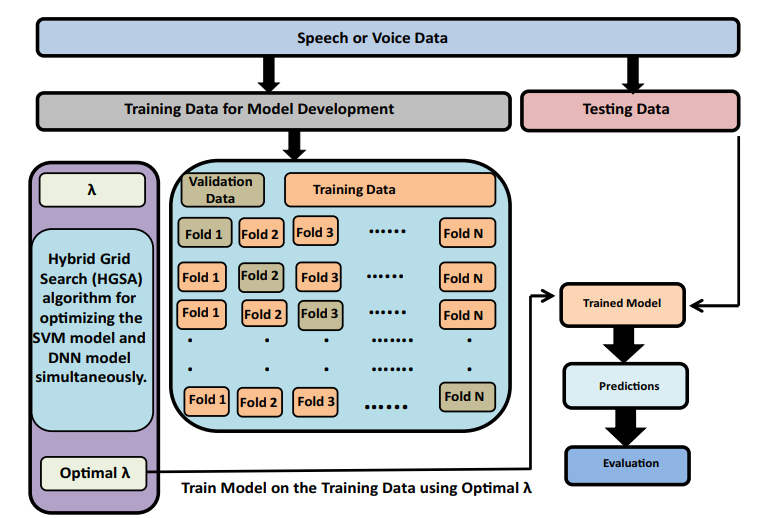
\includegraphics[width=\textwidth]{A1 - M.png}
    \caption{Metodología empleada para la detección de Parkinson utilizando el refinamiento de características con SVM regularizado y DNN.}
    \label{fig:metodologia}
\end{figure}

Para validar los modelos, el estudio implementó tanto la validación cruzada "leave-one-subject-out" (LOSO) como la validación cruzada k-fold. Estos métodos ayudan a reducir el sesgo en los datos y mejorar la generalización del modelo. La optimización de los hiperparámetros se llevó a cabo mediante una búsqueda aleatoria usando un híbrido de SVM y DNN, lo cual permitió ajustar los modelos para clasificar las muestras vocales de manera más precisa. La implementación se realizó en **Python**, utilizando librerías como **Scikit-learn** para aplicar SMOTE y realizar la selección de características, mientras que el ajuste de hiperparámetros se realizó con **RandomizedSearchCV**. Además, el procesamiento acústico de los datos se llevó a cabo en software especializado como **Praat**.

En cuanto a los resultados, el modelo propuesto alcanzó una precisión del 100\% en la validación LOSO y del 97.5\% en la validación k-fold en ambos conjuntos de datos, superando las técnicas tradicionales en la detección de PD. Estos resultados destacan el potencial de los modelos basados en voz como un método no invasivo, accesible y preciso para mejorar la intervención temprana en pacientes con Parkinson. A continuación, se presentan los resultados obtenidos para ambos conjuntos de datos:

\begin{figure}[H]
    \centering
    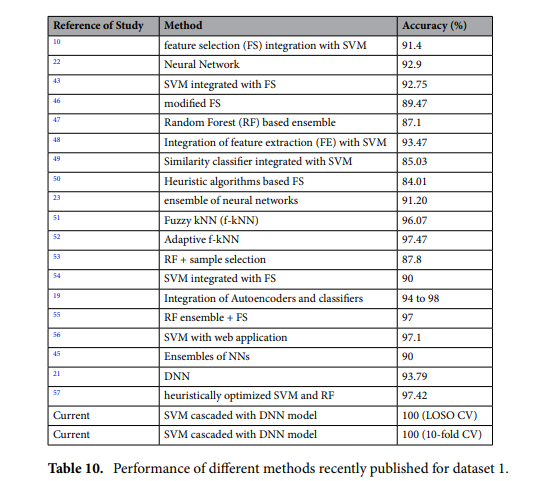
\includegraphics[width=\textwidth]{A1 - b1 .png}
    \caption{Resultados utilizando el primer conjunto de datos.}

    \label{fig:resultados_loso}
\end{figure}

\begin{figure}[H]
    \centering
    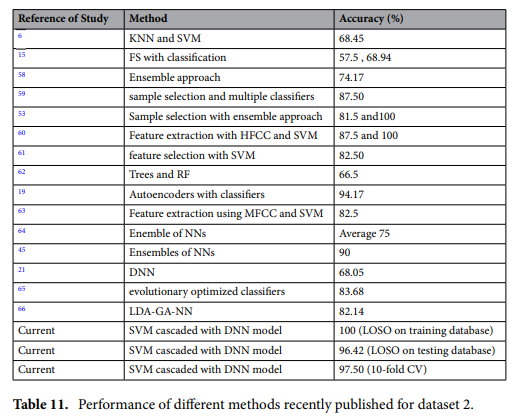
\includegraphics[width=\textwidth]{A1 - b2.png}
    \caption{Resultados utilizando el segundo conjunto de datos.}
    \label{fig:resultados_kfold}
\end{figure}

\subsection{Detection of Parkinson Disease Using Multiclass Machine Learning Approach (Srinivasan et al., 2024)}

Este estudio exploró la detección de la Enfermedad de Parkinson (PD) utilizando características vocales de grabaciones de voz, con el fin de desarrollar un método no invasivo que permita identificar esta condición de manera temprana y precisa. Para esto, se utilizó un conjunto de datos de la Universidad de California en Irvine (UCI), compuesto por 195 grabaciones de voz de 31 personas (23 diagnosticadas con Parkinson y 8 controles sanos). Las grabaciones incluyeron fonaciones sostenidas de la vocal "a" y se analizaron para extraer 22 características vocales biomédicas, tales como frecuencia fundamental (pitch), variaciones en frecuencia (jitter), variaciones en amplitud (shimmer), y la relación armónico-ruido, las cuales son indicadores significativos de disfunción vocal asociada a PD. El rango de edad de los sujetos variaba entre 46 y 85 años, y en los pacientes con PD, el tiempo desde el diagnóstico oscilaba entre 1 y 28 años.

\begin{figure}[H]
    \centering
    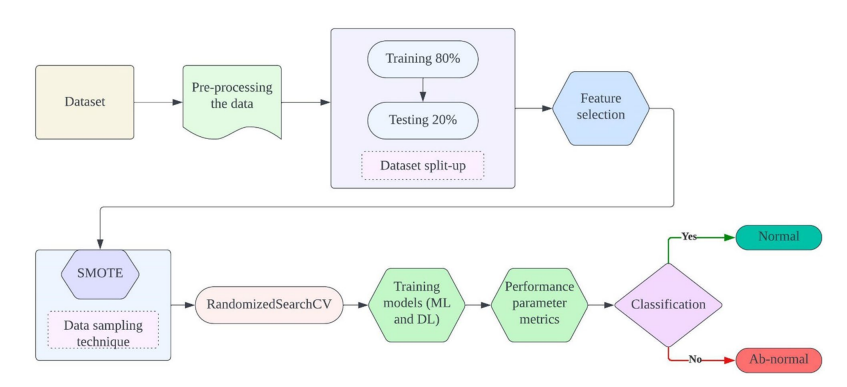
\includegraphics[width=\textwidth]{A2 - M.png}
    \caption{Metodología utilizada en la detección de Parkinson mediante el enfoque multiclasificación. Fuente: Srinivasan et al. (2024).}
    \label{fig:metodologia_multiclasificacion}
\end{figure}

En cuanto a la metodología, se aplicaron técnicas avanzadas de procesamiento y modelado de datos. Primero, para abordar el desbalance en las clases (mayor número de casos de PD que de controles sanos), se utilizó el Synthetic Minority Over-sampling Technique (SMOTE), que genera muestras sintéticas para la clase minoritaria y permite entrenar los modelos de manera más equilibrada. Además, se empleó Recursive Feature Elimination (RFE) para seleccionar las características más relevantes, optimizando así el rendimiento de los modelos y reduciendo la posibilidad de sobreajuste. Para el análisis, se implementaron varios algoritmos de machine learning y deep learning, incluyendo K-Nearest Neighbor (KNN), Support Vector Machine (SVM), Random Forest (RF), Decision Tree (DT), y una Red Neuronal de Propagación hacia Adelante (FNN). Cada modelo fue optimizado mediante RandomizedSearchCV, que explora de manera eficiente combinaciones de hiperparámetros, y se evaluaron con métricas de precisión, recall, precisión y puntuación F1 para asegurar un desempeño robusto.

\begin{figure}[H]
    \centering
    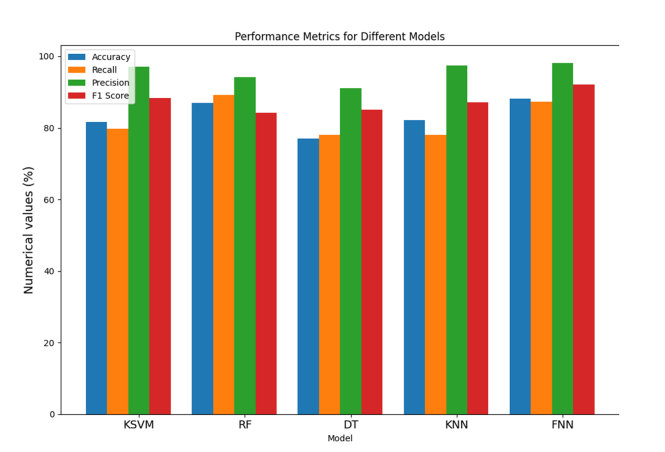
\includegraphics[width=\textwidth]{A2 - r2.png}
    \caption{Resultados obtenidos por cada modelo en el enfoque multiclasificación. Fuente: Srinivasan et al. (2024).}
    \label{fig:resultados_multiclasificacion}
\end{figure}

Los resultados mostraron que la Red Neuronal de Propagación hacia Adelante (FNN) alcanzó los mejores resultados en comparación con otros modelos, logrando una precisión del 99.11\%, un recall del 98.78\%, una precisión del 99.96\% y una puntuación F1 de 99.23\%. Otros modelos como el KSVM y el Random Forest también demostraron un rendimiento alto, con precisiones de 95.89\% y 93.12\%, respectivamente. Estos hallazgos sugieren que el modelo FNN tiene un gran potencial para identificar de manera precisa los casos de PD con una baja tasa de falsos positivos, lo cual es esencial para un diagnóstico confiable.


\subsection{Developing System-based Voice Features for Detecting Parkinson’s Disease Using Machine Learning Algorithms (Al-Nefaie et al., 2024)}

El estudio se centra en el desarrollo de algoritmos de machine learning (ML) para mejorar la detección de la enfermedad de Parkinson (PD) a través del análisis de voz. La investigación fue llevada a cabo por Abdullah H. Al-Nefaie, Theyazn H. H. Aldhyani y Deepika Koundal, y publicada en el \textit{Journal of Disability Research} en 2024.

La investigación empleó varios algoritmos de ML, incluidos k-nearest neighbors (k-NN), support vector machines (SVM), random forest (RF), logistic regression (LR) y AdaBoost, para analizar un conjunto de datos de muestras de voz de individuos con PD y controles sanos. El conjunto de datos consistió en 195 muestras de voz, con 147 de pacientes con PD y 48 de individuos sanos, abarcando 23 características distintas.

\begin{figure}[H]
    \centering
    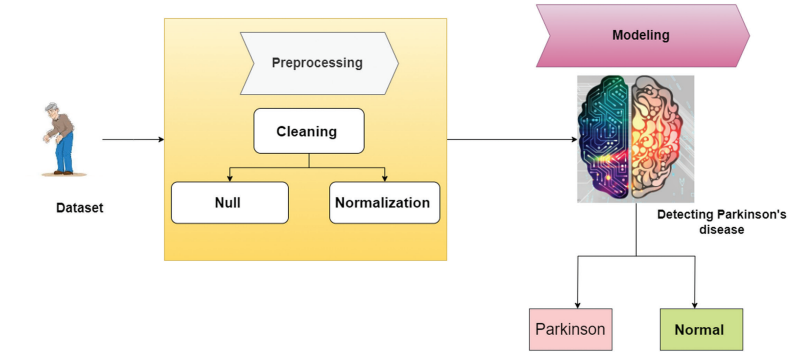
\includegraphics[width=\textwidth]{A3 - 1.png}
    \caption{Metodología utilizada en el desarrollo de características vocales para la detección de la enfermedad de Parkinson. Fuente: Al-Nefaie et al. (2024).}
    \label{fig:metodologia_sistema_vocal}
\end{figure}


El estudio encontró que los modelos SVM y RF lograron las tasas de precisión más altas del 95\%, mientras que k-NN alcanzó el 92\%, AdaBoost el 93\% y LR el 86\%. Los resultados indican que estas técnicas de ML pueden distinguir eficazmente entre individuos con PD y sanos, lo que potencialmente puede ayudar en el diagnóstico y tratamiento temprano.

\begin{table}[H]
\centering
\caption{Resultados de precisión de los modelos de machine learning.}
\label{tab:accuracy_results}
\begin{tabular}{|l|c|}
\hline
\textbf{Modelo} & \textbf{Precisión (\%)} \\ \hline
LR (Regresión Logística) & 86 \\ \hline
k-NN (K-Vecinos Más Cercanos) & 92 \\ \hline
SVM (Máquinas de Vectores de Soporte) & 95 \\ \hline
RF (Bosques Aleatorios) & 95 \\ \hline
AdaBoost Boosting & 93 \\ \hline
\end{tabular}
\begin{flushleft}
\footnotesize \textbf{Fuente:} Elaboración propia basada en Al-Nefaie et al. (2024).
\end{flushleft}
\end{table}



Los hallazgos destacan la importancia de la detección temprana de PD, lo que puede llevar a una mejor gestión de los síntomas y una mejora en la calidad de vida de los pacientes. El estudio sugiere que el sistema basado en ML propuesto podría servir como una herramienta confiable para los profesionales de la salud, abordando los desafíos actuales en el diagnóstico de PD.
La investigación demuestra el potencial de utilizar algoritmos de ML para la detección temprana de la enfermedad de Parkinson a través del análisis de voz, con tasas de precisión prometedoras que podrían mejorar los procesos de diagnóstico en entornos clínicos. Trabajos futuros podrían explorar conjuntos de datos adicionales y técnicas para mejorar aún más la precisión de clasificación.

\subsection{Use of Laughter for the Detection of Parkinson’s Disease (Terriza et al., 2022)}

La enfermedad de Parkinson (PD) es un trastorno neurodegenerativo incurable que afecta a más de 10 millones de personas en todo el mundo. La detección temprana y una evaluación precisa de la enfermedad son esenciales para implementar tratamientos que ralenticen el avance de los síntomas y mejoren la calidad de vida de los pacientes.

En este contexto, es crucial desarrollar sistemas de apoyo a la decisión clínica que permitan un diagnóstico temprano, eficiente y fiable. Este trabajo, realizado por Terriza et al. (2022), propone un estudio de viabilidad para un sistema de apoyo clínico basado en el análisis de las características acústicas de la risa para diferenciar entre individuos sanos y pacientes con PD.

El estudio utilizó coeficientes cepstrales para analizar risas de 120 sujetos (60 sanos y 60 con PD) y aplicó algoritmos de machine learning como Random Forest, k-Nearest Neighbors y SVM para la clasificación. La evaluación se llevó a cabo utilizando una base de datos clínica obtenida en Zaragoza, España, con 20,000 muestras de risa generadas a partir de un conjunto inicial de 120 risas. Las herramientas utilizadas incluyeron MATLAB y WEKA para el procesamiento y la clasificación. 

Los resultados demostraron una tasa de precisión del 83\% y un valor de AUC de 0.86 en la clasificación de las risas. Esto respalda la viabilidad de emplear la risa como un biomarcador acústico prometedor para la detección temprana de PD. Implementar un sistema de apoyo a la decisión basado en estas técnicas podría mejorar significativamente el diagnóstico y tratamiento, reduciendo costos y mejorando las condiciones de vida de las personas afectadas.

\begin{figure}[H]
    \centering
    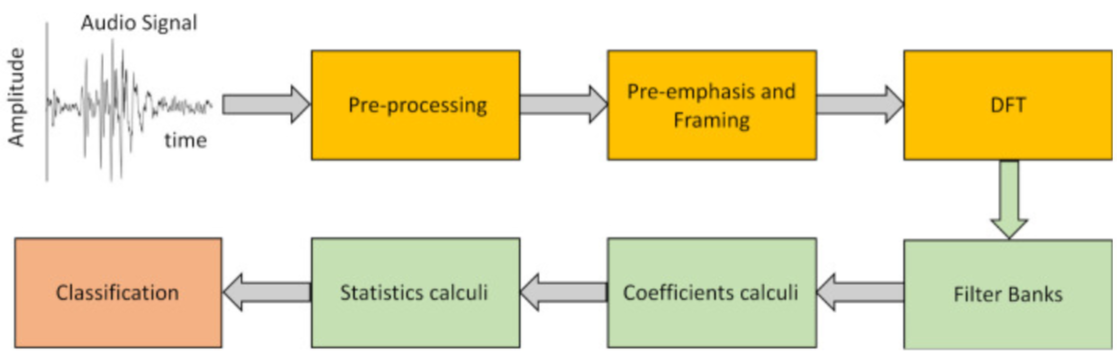
\includegraphics[width=\textwidth]{A4 - 1.png}
    \caption{Metodología utilizada para el estudio (Terriza et al., 2022).}
    \label{fig:metodologia_risa}
\end{figure}

\begin{figure}[H]
    \centering
    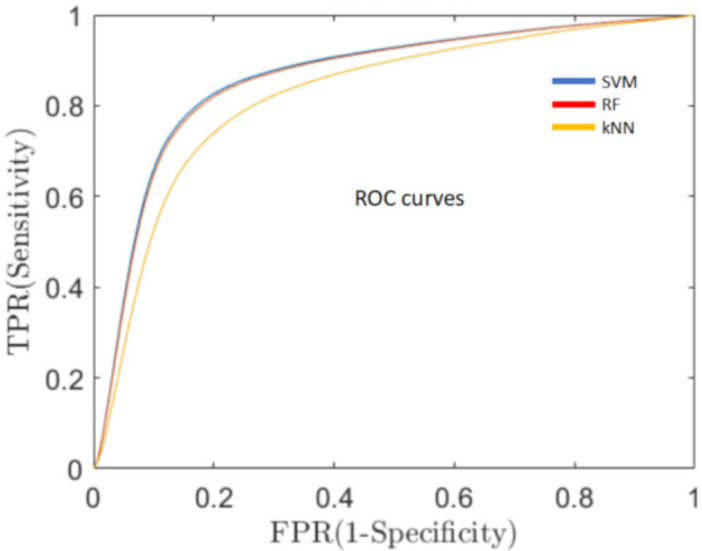
\includegraphics[width=\textwidth]{A4 - 2 .png}
    \caption{Curva ROC - Resultados (Terriza et al., 2022).}
    \label{fig:resultados_risa}
\end{figure}

\subsection{Accessible, At-Home Detection of Parkinson’s Disease via Multi-task Video Analysis (Islam et al., 2024)}

La enfermedad de Parkinson (PD) a menudo es subdiagnosticada debido al acceso limitado a la atención neurológica, particularmente en regiones desatendidas. Este estudio introduce un enfoque novedoso para la detección remota de PD mediante el desarrollo de un método de detección que utiliza el análisis de videos en el hogar con la Red de Fusión Calibrada por Incertidumbre (UFNet), la cual combina tareas de golpeteo de dedos, sonrisa y habla. Se recopilaron videos de 845 participantes, de los cuales 272 estaban diagnosticados con PD, abarcando 1102 sesiones de video divididas en 60\% para entrenamiento, 20\% para la selección del modelo y 20\% para evaluación. Las grabaciones se obtuvieron a través de webcams, y cada tarea se analizó utilizando Monte Carlo Dropout para mejorar la precisión, permitiendo que UFNet fusione características de todas las tareas. La creación del conjunto de datos presenta el primer conjunto de datos de video de gran escala y múltiples tareas para la detección de PD, que estará disponible en forma de características extraídas para proteger la privacidad del paciente. El rendimiento del modelo UFNet logró una precisión de 88.0\% con un margen de error de ±0.3\% y un AUROC de 93.0\% ± 0.2\%, superando significativamente a los modelos de tarea única y otros modelos de fusión multimodal. Los modelos específicos de la tarea indicaron que la tarea de habla fue la más efectiva para clasificar a individuos con y sin PD, logrando una precisión de 84.5\% ± 0.3\%. La combinación de las tres tareas en el modelo UFNet resultó en métricas mejoradas, incluida una precisión de 87.3\% ± 0.4\% y un AUROC de 92.8\% ± 0.2\%. El modelo demostró no tener sesgo significativo entre subgrupos de sexo y etnia, aunque el rendimiento varió según el grupo de edad. Los hallazgos sugieren que el análisis de video puede proporcionar un medio rentable y accesible para el cribado de PD, especialmente beneficioso para individuos en áreas remotas. El estudio enfatiza la importancia de utilizar un enfoque multimodal para capturar los diversos síntomas de la PD, que pueden no ser evaluados adecuadamente a través de modelos de tarea única. Sin embargo, el rendimiento del modelo fue menos robusto para los grupos de edad más jóvenes y mayores, probablemente debido a la subrepresentación en el conjunto de datos. Además, se observaron desafíos como el incumplimiento de las instrucciones de la tarea y el ruido de fondo durante la grabación de video, lo que podría afectar la calidad de los datos. Esta investigación resalta el potencial de los modelos de aprendizaje automático para la detección remota de PD utilizando tecnología simple como webcams y micrófonos, allanando el camino para aplicaciones más amplias de tele-neurología. El estudio tiene como objetivo facilitar la intervención temprana y mejorar la calidad de vida de los individuos en riesgo de PD.

\begin{figure}[H]
    \centering
    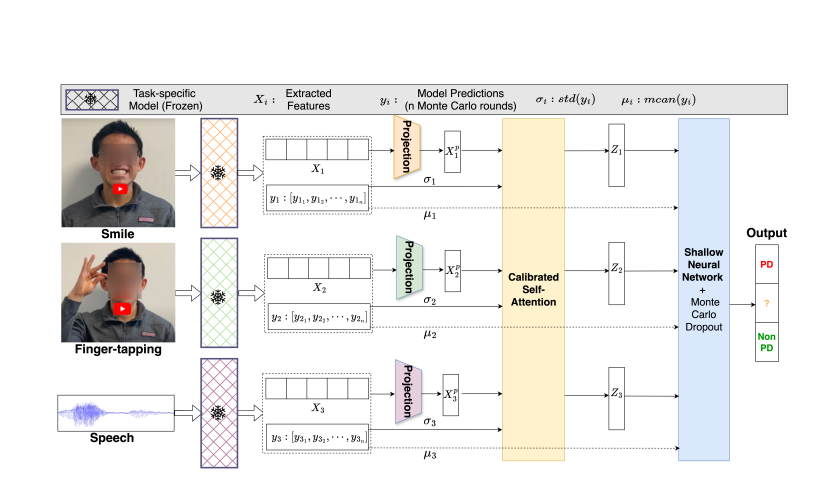
\includegraphics[width=\textwidth]{A5 - 1.png}
    \caption{Metodología utilizada en el análisis de video para la detección de la enfermedad de Parkinson. Fuente: Islam, Md Saiful et al. (2024). Accessible, At-Home Detection of Parkinson's Disease via Multi-task Video Analysis. \textit{arXiv:2406.14856}.}
    \label{fig:metodologia_video}
\end{figure}



\begin{table}[H]
\centering
\caption{Resultados detallados de evaluación de modelos de fusión.}
\label{tab:fusion_models_results}
\resizebox{\textwidth}{!}{%
\begin{tabular}{|l|c|c|c|c|c|c|c|c|c|c|}
\hline
\textbf{Modelo} & \textbf{Precisión (\%)} & \textbf{Precisión Balanceada (\%)} & \textbf{AUROC} & \textbf{AUPRC} & \textbf{\textit{F1}-Score} & \textbf{PPV (Precisión)} & \textbf{NPV} & \textbf{Sensibilidad (\%)} & \textbf{Especificidad (\%)} & \textbf{Cobertura (\%)} \\ \hline
Majority Voting & 85.3 & 83.9 & 89.6 & 78.0 & 78.2 & 80.0 & 87.9 & 76.5 & 89.9 & - \\ \hline
Neural Late Fusion & 84.1 $\pm$ 0.4 & 81.3 $\pm$ 4.8 & 91.7 $\pm$ 2.2 & 86.7 $\pm$ 3.1 & 73.2 $\pm$ 8.3 & 73.5 $\pm$ 7.5 & 89.2 $\pm$ 3.3 & 76.3 $\pm$ 9.4 & 88.2 $\pm$ 2.7 & - \\ \hline
Early Fusion Baseline & 83.6 $\pm$ 0.6 & 81.8 $\pm$ 0.7 & 91.0 $\pm$ 0.2 & 85.8 $\pm$ 0.4 & 76.7 $\pm$ 0.7 & 75.4 $\pm$ 1.1 & 88.3 $\pm$ 0.4 & 78.1 $\pm$ 0.9 & 86.5 $\pm$ 0.8 & - \\ \hline
Hybrid Fusion Baseline & 84.1 $\pm$ 0.3 & 82.4 $\pm$ 0.4 & 91.4 $\pm$ 0.2 & 86.5 $\pm$ 0.3 & 77.3 $\pm$ 0.4 & 76.2 $\pm$ 0.4 & 88.5 $\pm$ 0.3 & 78.6 $\pm$ 0.6 & 87.0 $\pm$ 0.6 & - \\ \hline
\textit{UFNet} - Early Fusion & 86.7 $\pm$ 0.5 & 85.8 $\pm$ 0.5 & 92.7 $\pm$ 0.3 & 86.2 $\pm$ 0.5 & 79.9 $\pm$ 0.8 & 83.3 $\pm$ 0.7 & 88.3 $\pm$ 0.6 & 76.9 $\pm$ 1.4 & 91.9 $\pm$ 0.4 & - \\ \hline
\textit{UFNet} - Early Fusion (withhold uncertain preds) & 87.5 $\pm$ 0.4 & 86.5 $\pm$ 0.5 & 92.9 $\pm$ 0.3 & 86.4 $\pm$ 0.7 & 80.7 $\pm$ 0.8 & 84.0 $\pm$ 0.7 & 89.1 $\pm$ 0.6 & 77.7 $\pm$ 1.4 & 92.4 $\pm$ 0.4 & 97.4 $\pm$ 0.3 \\ \hline
\textit{UFNet} - Hybrid Fusion & 87.3 $\pm$ 0.4 & 86.4 $\pm$ 0.4 & 92.8 $\pm$ 0.2 & 86.3 $\pm$ 0.5 & 81.0 $\pm$ 0.6 & 83.8 $\pm$ 0.5 & 89.0 $\pm$ 0.4 & 78.4 $\pm$ 1.0 & 92.0 $\pm$ 0.3 & - \\ \hline
\textit{UFNet} - Hybrid Fusion (withhold uncertain preds) & \textbf{88.0 $\pm$ 0.3} & \textbf{87.1 $\pm$ 0.4} & \textbf{93.0 $\pm$ 0.2} & \textbf{86.5 $\pm$ 0.6} & \textbf{81.8 $\pm$ 0.6} & \textbf{84.6 $\pm$ 0.5} & \textbf{89.7 $\pm$ 0.4} & \textbf{79.3 $\pm$ 0.9} & \textbf{92.6 $\pm$ 0.2} & \textbf{97.8 $\pm$ 0.3} \\ \hline
\end{tabular}%
}
\end{table}



\subsection{Voice Biomarkers for Parkinson's Disease Prediction Using Machine Learning Models with Improved Feature Reduction Techniques (Chintalapudi et al., 2023)}


Este estudio explora el uso de biomarcadores de voz para la predicción de la enfermedad de Parkinson (PD) utilizando modelos de machine learning (ML) y técnicas avanzadas de reducción de características. Las grabaciones de voz fueron empleadas como biomarcadores junto con el Synthetic Minority Over-sampling Technique (SMOTE) para mejorar la precisión en la detección de PD. Tres modelos de ML, Support Vector Machine (SVM), K-nearest Neighbors (KNN) y Random Forest (RF), fueron evaluados en términos de precisión, sensibilidad y área bajo la curva (AUC), destacando el modelo de RF con la mayor precisión.

El enfoque experimental combina técnicas de reducción de características, como el análisis de componentes principales (PCA), con SMOTE para equilibrar el conjunto de datos. Tras el preprocesamiento, los modelos se entrenaron usando validación cruzada de 10 pliegues.

\begin{figure}[H]
    \centering
    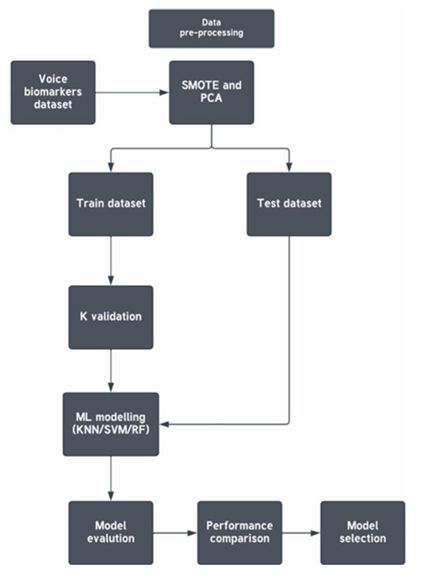
\includegraphics[width=0.8\textwidth]{A6 - 1.png}
    \caption{Metodología para la clasificación de PD. Fuente: Chintalapudi, Nalini et al. (2023). Voice Biomarkers for Parkinson's Disease Prediction Using Machine Learning Models with Improved Feature Reduction Techniques. \textit{Journal of Data Science and Intelligent Systems}}
\end{figure}


\begin{table}[H]
\centering
\caption{Métricas de desempeño entre los modelos de ML.}
\label{table:metrics_ml}
\begin{tabular}{|c|c|c|c|c|}
\hline
\textbf{Algorithm} & \textbf{Precision} & \textbf{Recall} & \textbf{F1 Score} & \textbf{AUC} \\ \hline
SVM                & 0.92               & 0.88            & 0.86              & 0.91         \\ \hline
KNN                & 0.84               & 0.91            & 0.92              & 0.93         \\ \hline
RF                 & 1.00               & 0.96            & 0.98              & 0.96         \\ \hline
\end{tabular}
\end{table}




\subsection{Parkinson’s Disease Detection Using Filter Feature Selection and a Genetic Algorithm with Ensemble Learning (Ali et al., 2023)}


Este estudio presenta un enfoque para la detección de la enfermedad de Parkinson (PD) utilizando selección de características con filtros y algoritmos genéticos combinados con métodos de aprendizaje en conjunto (ensemble learning). Se utilizaron grabaciones de voz de pacientes con PD y personas sanas para extraer atributos relevantes y entrenar varios modelos de clasificación. Los algoritmos de clasificación incluyeron árboles de decisión, random forest y XGBoost, logrando una precisión muy alta en uno de los conjuntos de datos analizados. Se implementaron métodos de aprendizaje en conjunto como votación y apilamiento para mejorar el rendimiento de los modelos.
 La metodología incluye la selección de características mediante la eliminación de aquellas con variación cuasi-constante y la aplicación de un algoritmo genético para optimizar aún más la selección de características en combinación con técnicas de aprendizaje en conjunto.

\begin{figure}[H]
    \centering
    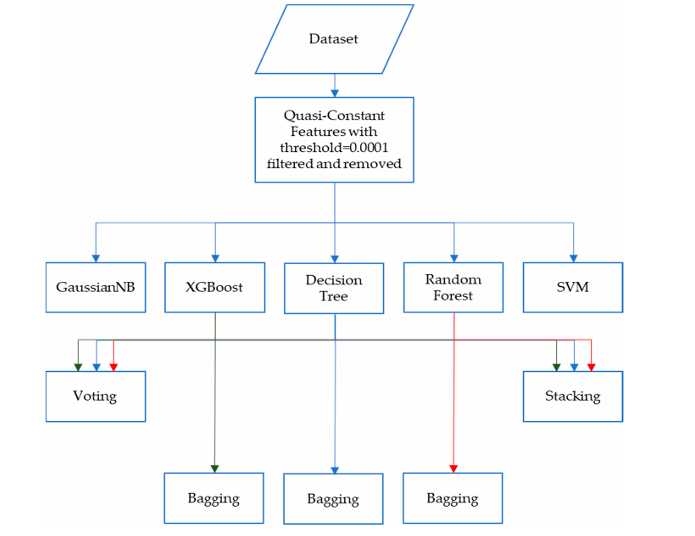
\includegraphics[width=0.8\textwidth]{A7 - 1.png} % Reemplaza "A7 - 1.png" con el nombre de tu archivo de imagen
    \caption{Metodología del estudio para la detección de PD. Fuente: Ali, A. M., Salim, F., & Saeed, F. (2023)}
\end{figure}


 Los resultados indicaron que los métodos de aprendizaje en conjunto, en particular la votación y el apilamiento, mejoraron significativamente la precisión de los modelos, alcanzando una precisión perfecta en uno de los conjuntos de datos.



\begin{table}[h!]
\centering
\begin{tabular}{lcc}
\toprule
\textbf{Classification Model} & \textbf{Dataset 1} & \textbf{Dataset 2} \\
\midrule
GaussianNB          & 91.83 & 77.63 \\
SVM                 & 81.63 & 77.63 \\
Decision Tree-entropy & 81.63 & 76.65 \\
Decision Tree-Gini  & 81.63 & 74.34 \\
Random Forest       & 83.67 & 74.34 \\
XGBoost             & 87.75 & 76.97 \\
Logistic Regression & 89.79 & 76.97 \\
\bottomrule
\end{tabular}
\caption{Accuracy (in \%) after Filter Feature Selection}
\label{tab:accuracy_results}
\end{table}








\section{Bases Teóricas}

\subsection{Machine Learning}
El Machine Learning, o aprendizaje automático, se ha convertido en un componente fundamental en la forma en que manejamos y analizamos datos en diversas disciplinas, incluida la medicina. A grandes rasgos, se refiere a la capacidad de las computadoras para aprender de los datos, ajustando su comportamiento sin la necesidad de ser programadas de manera explícita para cada tarea. Esto es especialmente útil en campos donde los datos son complejos y abundantes. Dentro de este ámbito, se pueden distinguir tres grandes categorías: el aprendizaje supervisado, no supervisado y por refuerzo. El aprendizaje supervisado es particularmente relevante en nuestro estudio, ya que se basa en la utilización de conjuntos de datos etiquetados para entrenar modelos que luego pueden hacer predicciones o clasificaciones sobre datos nuevos y no vistos. Por ejemplo, en el diagnóstico de enfermedades como el Parkinson, se busca identificar patrones en las características vocales de los pacientes que podrían indicar la presencia de la enfermedad. Esto es crucial porque un diagnóstico temprano puede mejorar significativamente la calidad de vida de los afectados, permitiendo iniciar tratamientos más efectivos en etapas iniciales (Bishop, 2006).

\subsection{Deep Learning}
Dentro del vasto campo del Machine Learning, una técnica que ha cobrado un protagonismo notable es el Deep Learning. Esta técnica se basa en la utilización de redes neuronales profundas, que son modelos computacionales inspirados en el funcionamiento del cerebro humano. Estas redes están compuestas por múltiples capas de neuronas artificiales que procesan la información de manera jerárquica. En el contexto del análisis de voz, el Deep Learning es especialmente potente, ya que permite extraer características de alto nivel a partir de señales acústicas complejas. Estudios recientes han demostrado que los modelos de Deep Learning pueden superar a los métodos tradicionales en tareas de clasificación de audio, ofreciendo una precisión mucho mayor en el diagnóstico temprano de enfermedades como el Parkinson (LeCun et al., 2015). Esto significa que podemos identificar patrones que antes eran invisibles, lo que representa un gran avance en la búsqueda de diagnósticos más efectivos.

\subsection{Transfer Learning}
El Transfer Learning, o aprendizaje por transferencia, es una estrategia que permite a los modelos de Machine Learning aprovechar el conocimiento que han adquirido de una tarea previa para mejorar su rendimiento en una nueva tarea. Esto es particularmente útil en el ámbito de la medicina, donde a menudo no contamos con suficientes datos para entrenar modelos robustos desde cero. Por ejemplo, un modelo que ha sido preentrenado en un gran conjunto de datos de voz puede ser ajustado para identificar características específicas de la voz de pacientes con Parkinson. Esta metodología no solo ahorra tiempo y recursos, sino que también mejora la precisión del modelo y reduce el riesgo de sobreajuste (Pan y Yang, 2010). En otras palabras, se trata de aprender de experiencias pasadas para aplicarlas de forma efectiva a nuevos desafíos.

\subsection{Data Augmentation}
Uno de los problemas comunes que enfrentamos en la investigación médica es la escasez de datos. Para abordar esto, recurrimos a técnicas de **aumento de datos** (data augmentation), que permiten generar variaciones en nuestros datos de entrenamiento sin la necesidad de recopilar nuevos ejemplos. En el análisis de voz, esto puede implicar modificaciones en la velocidad de reproducción, cambios en el tono, o la inclusión de ruido de fondo. Estas técnicas son fundamentales, ya que permiten que el modelo se vuelva más robusto y generalice mejor en situaciones del mundo real, algo esencial para la detección temprana de la enfermedad de Parkinson (Shorten y Khoshgoftaar, 2019). Imaginemos que un modelo puede escuchar una grabación de voz de un paciente y, gracias a estas variaciones, aprender a reconocer la enfermedad incluso cuando la grabación no es perfecta. Esto puede hacer una gran diferencia en el diagnóstico.

\subsection{Análisis Acústico}
El análisis acústico es un aspecto fundamental en la evaluación de las características vocales. Utiliza diversas métricas para cuantificar propiedades de la voz, como la frecuencia, la amplitud y la variabilidad. Entre estas métricas, destacan el **jitter** y el **shimmer**. El jitter se refiere a la variación en el período de las ondas de sonido, mientras que el shimmer mide la variación en la amplitud de la voz. Estas fluctuaciones pueden ser indicadores clave de alteraciones en la voz asociadas con el Parkinson. De hecho, varios estudios han demostrado que los pacientes con esta enfermedad tienden a exhibir niveles más altos de jitter y shimmer, lo que facilita la identificación temprana de la condición (Murray, 2000). Así que, al analizar las grabaciones de voz, podemos obtener información valiosa sobre el estado de salud de una persona, casi como si estuviéramos leyendo su historia clínica a través de su voz.

\subsection{Características Vocales en Pacientes con Parkinson}
La enfermedad de Parkinson se asocia con varios cambios en las características vocales que pueden ser analizados para ayudar en el diagnóstico. Los pacientes suelen presentar una voz más débil y monótona, con dificultades para modular el tono. Esto no solo afecta la calidad de la voz, sino que también puede impactar la capacidad de comunicación del paciente. Reconocer estas características vocales es esencial, ya que su identificación temprana puede conducir a intervenciones más efectivas y mejorar la calidad de vida de los pacientes (Duffy, 2013). En algunos casos, una simple conversación puede revelar mucho más sobre la salud de una persona de lo que se podría imaginar.

\subsection{Algoritmos de Clasificación}
En nuestra búsqueda por lograr un diagnóstico preciso, diversos algoritmos de clasificación son utilizados. Entre los más destacados se encuentran el **Support Vector Machine (SVM), KNN y AdaBoost y Stacking. El SVM es un potente algoritmo que encuentra un hiperplano en un espacio multidimensional que separa las diferentes clases de datos. Por otro lado, Random Forest construye múltiples árboles de decisión y fusiona sus resultados, lo que lo hace muy eficaz para manejar conjuntos de datos grandes y complejos. Finalmente, AdaBoost se utiliza para mejorar la precisión de los modelos combinando múltiples clasificadores débiles en un único clasificador fuerte. Estas técnicas han demostrado ser efectivas en la identificación de patrones en las voces de pacientes con Parkinson, contribuyendo así al diagnóstico precoz (Zhang et al., 2018). Cada uno de estos algoritmos tiene sus propias fortalezas y debilidades, y elegir el adecuado puede ser la clave para lograr un diagnóstico exitoso.

\subsection{Diagnóstico No Invasivo}
El diagnóstico no invasivo se refiere a técnicas que no requieren procedimientos invasivos o la manipulación directa del cuerpo del paciente. En el contexto del Parkinson, el análisis de voz ofrece una alternativa prometedora para la detección temprana de la enfermedad. Al ser una técnica sencilla, económica y fácil de implementar, puede utilizarse en diversas configuraciones, desde consultorios médicos hasta entornos rurales donde el acceso a atención especializada es limitado. Implementar métodos de análisis de voz no solo puede mejorar el acceso al diagnóstico, sino que también fomenta la detección temprana y, por ende, intervenciones más efectivas (Morrison et al., 2019). Al final del día, se trata de encontrar formas de llegar a quienes más lo necesitan, y la tecnología puede ser un aliado valioso en este esfuerzo.

\subsection{Aplicaciones Prácticas de Machine Learning en el Diagnóstico de Parkinson}
A lo largo de los años, numerosos estudios han demostrado el potencial del **Machine Learning** en el diagnóstico de Parkinson a través del análisis de voz. Investigaciones recientes han utilizado diversas combinaciones de algoritmos y características vocales para lograr altas tasas de precisión en la identificación de la enfermedad. Estas aplicaciones prácticas no solo evidencian la viabilidad de este enfoque, sino que también resaltan la necesidad de seguir explorando y desarrollando herramientas de diagnóstico que aprovechen el poder de la inteligencia artificial para mejorar la atención médica (Tiwari et al., 2020). En un mundo donde la tecnología avanza a pasos agigantados, es emocionante pensar en las posibilidades que se abren para mejorar la vida de los pacientes.



\section{Marco Conceptual}


\subsection{Introducción a la Enfermedad de Parkinson}

La enfermedad de Parkinson es una de las enfermedades neurodegenerativas más comunes que afecta a millones de personas en todo el mundo. Se caracteriza por la degeneración progresiva de neuronas en la sustancia negra, una región del cerebro responsable de la producción de dopamina. Esta neurotransmisor es crucial para el control del movimiento, y su disminución causa una serie de síntomas motores y no motores que impactan significativamente la calidad de vida de los pacientes.

Los síntomas motores típicos incluyen temblores en reposo, rigidez muscular, bradicinesia (lentitud de movimientos) y problemas de equilibrio. A menudo, estos síntomas comienzan de forma leve y se vuelven más severos con el tiempo. Además, los pacientes pueden experimentar síntomas no motores como depresión, ansiedad, problemas cognitivos y alteraciones en la voz, que pueden pasar desapercibidos en las etapas iniciales de la enfermedad.

El diagnóstico temprano es fundamental, ya que permite implementar intervenciones terapéuticas que pueden retrasar la progresión de la enfermedad y mejorar la calidad de vida del paciente. En este contexto, el análisis de las características vocales se ha convertido en un área de interés para la detección temprana del Parkinson, dado que los cambios en la voz pueden ser indicativos de la presencia de la enfermedad.

\subsection{Variables de la Voz en Pacientes con Parkinson}

El análisis de la voz en pacientes con Parkinson se centra en diversas variables acústicas que pueden ser medidas y analizadas para identificar patrones asociados con la enfermedad. Algunas de estas variables incluyen:

\begin{itemize}
    \item Frecuencia Fundamental (F0): Esta medida representa el tono de la voz y se refiere a la frecuencia más baja de vibración de las cuerdas vocales. Los pacientes con Parkinson a menudo presentan una frecuencia fundamental alterada, manifestando un tono más grave o inestable.

    \item Intensidad: Se refiere al volumen de la voz. Los estudios han demostrado que muchos pacientes con Parkinson pueden experimentar una disminución en la intensidad vocal, lo que resulta en un habla más suave o susurrante.

    \item Duración: La duración se relaciona con el tiempo que se toma para producir sonidos o palabras, así como la longitud de las pausas. Los pacientes pueden mostrar una mayor variabilidad en la duración de los fonemas, lo que puede dificultar la fluidez del habla.

    \item Jitter: Este es un índice que mide la variabilidad en la frecuencia fundamental de la voz. Un mayor jitter indica una inestabilidad en el tono, lo que es común en pacientes con trastornos de la voz, incluida la enfermedad de Parkinson.

    \item Shimmer: Similar al jitter, el shimmer mide la variabilidad en la amplitud de la señal vocal. Un aumento en el shimmer puede reflejar una inconsistencia en la intensidad del habla, un síntoma que puede ser observable en pacientes con Parkinson.
\end{itemize}

\subsection{Jitter y Shimmer}

El jitter y el shimmer son parámetros acústicos críticos en el análisis de la voz y se pueden calcular a través de las siguientes fórmulas.

\subsubsection{Jitter}

El jitter puede cuantificarse usando la siguiente fórmula:

\begin{equation}
    Jitter = \frac{1}{N-1} \sum_{i=1}^{N-1} \left| \frac{F0_{i+1} - F0_{i}}{F0_{i}} \right| \times 100
\end{equation}

donde \(F0\) representa la frecuencia fundamental medida en Hertz (Hz), y \(N\) es el número total de muestras. Este cálculo proporciona un porcentaje que representa la variabilidad en la frecuencia vocal. Valores altos de jitter indican una mayor inestabilidad en la producción del tono vocal, lo cual es común en los pacientes con Parkinson.

\subsubsection{Shimmer}

El shimmer, por otro lado, se mide como sigue:

\begin{equation}
    Shimmer = \frac{1}{N-1} \sum_{i=1}^{N-1} \left| \frac{A_{i+1} - A_{i}}{A_{i}} \right| \times 100
\end{equation}

donde \(A\) es la amplitud de la señal en un tiempo dado, expresada en decibelios (dB). Al igual que el jitter, el shimmer también se expresa como un porcentaje. Un mayor shimmer sugiere inconsistencias en la intensidad vocal, que pueden ser un indicativo de problemas en la musculatura vocal o el control neuromuscular en pacientes con Parkinson.

\subsection{Introducción al Aprendizaje Automático}

El aprendizaje automático (machine learning) es un campo de la inteligencia artificial que se centra en el desarrollo de algoritmos y modelos que permiten a las computadoras aprender de datos. A través de técnicas avanzadas, las máquinas pueden identificar patrones, realizar predicciones y mejorar su rendimiento con el tiempo sin ser explícitamente programadas para cada tarea.

El aprendizaje automático se clasifica generalmente en tres categorías:

\begin{itemize}
    \item Aprendizaje Supervisado: En este enfoque, los modelos se entrenan utilizando conjuntos de datos etiquetados, donde las entradas y salidas son conocidas. El objetivo es que el modelo aprenda a mapear entradas a salidas, de modo que pueda realizar predicciones sobre datos no vistos.

    \item Aprendizaje No Supervisado: A diferencia del aprendizaje supervisado, este método se utiliza en datos que no están etiquetados. El modelo busca identificar patrones o agrupaciones dentro de los datos, como segmentación de clientes o detección de anomalías.

    \item Aprendizaje por Refuerzo: Este tipo de aprendizaje se basa en la interacción del agente con un entorno. El agente toma decisiones y recibe recompensas o penalizaciones según sus acciones, lo que le permite aprender a optimizar su comportamiento para maximizar la recompensa total a lo largo del tiempo.
\end{itemize}

\subsection{Algoritmos de Aprendizaje Supervisado}

En el contexto de la detección temprana del Parkinson a través del análisis de voz, se utilizan varios algoritmos de aprendizaje supervisado, entre ellos:

\begin{itemize}
    \item Support Vector Machines (SVM): Este algoritmo busca encontrar el hiperplano que mejor separa las diferentes clases en el espacio de características. SVM es eficaz para problemas de clasificación y se utiliza frecuentemente en el análisis de voz para distinguir entre voces saludables y voces de pacientes con Parkinson.

    \item K-Nearest Neighbors (KNN): KNN es un método simple que clasifica una muestra basada en la mayoría de las clases de sus \(k\) vecinos más cercanos en el espacio de características. Este enfoque puede ser útil para problemas donde las características acústicas son similares entre diferentes clases.

    \item AdaBoost: AdaBoost es un algoritmo de ensemble que combina varios clasificadores débiles para crear un clasificador fuerte. Funciona asignando pesos a las instancias de entrenamiento, dándole mayor importancia a las que son más difíciles de clasificar.

    \item Stacking: Esta técnica combina múltiples modelos de aprendizaje automático para mejorar la precisión de las predicciones. Se entrena un modelo de nivel superior para hacer predicciones basadas en las salidas de varios modelos base.
\end{itemize}

El uso de estos algoritmos en el análisis de las características vocales de los pacientes con Parkinson ofrece una oportunidad valiosa para el desarrollo de sistemas de diagnóstico temprano que puedan facilitar una intervención oportuna y mejorar la calidad de vida de los pacientes.





\chapter{Metodología de la Investigación}

\section{ Diseño de la investigación}

Según trabajos previos en investigación científica, manipular y establecer una relación de causa-efecto entre variables independientes y dependientes es una característica fundamental de los diseños experimentales.

En esta investigación, se adopta un diseño experimental puro porque se busca establecer una relación entre los modelos y técnicas de aprendizaje supervisado (Machine Learning) y el prediagnóstico de Parkinson, utilizando el análisis de voz como fuente principal de datos. Las características acústicas de las grabaciones de voz serán analizadas y los modelos serán entrenados para clasificar las grabaciones como pertenecientes a pacientes con Parkinson o personas sanas.

\section{Tipo de la investigación}

El diseño experimental puro justifica que el tipo de investigación sea experimental, dado que la variable independiente (técnicas, modelos y herramientas de aprendizaje supervisado) será manipulada reiteradamente para evaluar su impacto en la variable dependiente.

Se aplicarán diferentes modelos de aprendizaje supervisado como Support Vector Machines (SVM), K-Nearest Neighbors (KNN), AdaBoost, Stacking y Deep Learning(CNN). Estos modelos serán optimizados y evaluados mediante métricas específicas para determinar su efectividad en el prediagnóstico del Parkinson. Además, se trabajará en la limpieza y transformación de los datos de audio para garantizar que las características extraídas sean representativas y relevantes para la tarea de clasificación.

\section{Enfoque de la investigación}

El enfoque cuantitativo es esencial en esta investigación porque permite representar las variables independientes y dependientes numéricamente. Las características acústicas extraídas de los audios (frecuencia, intensidad, jitter, shimmer, entre otras) serán evaluadas mediante herramientas estadísticas y algoritmos de aprendizaje supervisado.

\section{Población}
La población de esta investigación está conformada por grabaciones de voz de individuos diagnosticados con la enfermedad de Parkinson (EP) y de personas saludables. Estas grabaciones representan una fuente crucial para el análisis de patrones acústicos relacionados con la EP. La base de datos utilizada, conocida como el \textit{Oxford Parkinson's Disease Detection Dataset}, incluye datos biomédicos derivados de mediciones de voz. Este conjunto de datos contiene grabaciones de 31 individuos, de los cuales 23 tienen diagnóstico confirmado de EP, y 8 son individuos sanos de la ciudad de Londres.

\section{Muestra}
La muestra utilizada en este estudio consiste en 197 instancias correspondientes a grabaciones de voz incluidas en el \textit{Oxford Parkinson's Disease Detection Dataset}. Cada registro de la muestra contiene mediciones específicas de la voz, como frecuencias fundamentales (promedio, máximo y mínimo), variaciones en frecuencia y amplitud, y métricas no lineales de complejidad. Las grabaciones están correctamente etiquetadas para clasificar a los individuos como saludables (estatus = 0) o con EP (estatus = 1), lo que permite su uso en tareas de clasificación. Este conjunto de datos no presenta valores faltantes, garantizando su integridad para el análisis. 

La selección de esta muestra se fundamenta en la representatividad de las características acústicas y la diversidad de patrones vocales presentes en las grabaciones, lo que asegura un análisis robusto y aplicable al objetivo del prediagnóstico de Parkinson.

\subsection{Variables del la base de datos}
\begin{itemize}
    \item \textbf{name}: Esta variable corresponde al nombre del individuo, lo que no tiene un valor directo en el análisis de las características vocales. Sin embargo, puede ser utilizada para asociar las grabaciones con los pacientes específicos y mantener un seguimiento en el conjunto de datos. Es una variable categórica nominal que se utiliza solo como identificador para cada grabación.
    
    \item \textbf{MDVP:Fo (Hz)}: La frecuencia fundamental (Fo) es la frecuencia base a la que vibran las cuerdas vocales. Se mide en Hertzios (Hz). Es una medida importante de la tonalidad de la voz. Esta variable se utiliza para capturar el tono general de la voz, que en personas con Parkinson puede presentar una reducción en la variabilidad, mostrando una tonalidad más monótona.
    
    \item \textbf{MDVP:Fhi (Hz)}: La frecuencia fundamental máxima (Fhi) se refiere a la frecuencia más alta alcanzada durante la emisión vocal. Se utiliza para evaluar la flexibilidad vocal y el rango de modulación de la voz. Los pacientes con Parkinson pueden mostrar una limitación en el rango de frecuencias.
    
    \item \textbf{MDVP:Flo (Hz)}: La frecuencia fundamental mínima (Flo) corresponde a la frecuencia más baja alcanzada durante el habla. Esta variable complementa las otras mediciones de frecuencia para evaluar el rango completo de la frecuencia fundamental de la voz, que puede verse afectado por la enfermedad de Parkinson.
    
    \item \textbf{MDVP:Jitter (\%)}: El jitter es una medida de la variabilidad temporal en la frecuencia de la voz. Un alto jitter indica una mayor variabilidad en la frecuencia fundamental, lo cual es común en trastornos neurológicos como el Parkinson. Se utiliza como indicador de la irregularidad temporal en la voz, lo cual puede ser mayor en los pacientes con Parkinson debido a la alteración en el control motor fino.
    
    \item \textbf{MDVP:Jitter (Abs)}: El jitter absoluto es una medida similar al jitter en porcentaje, pero en unidades absolutas. Esta variable mide la variabilidad temporal de la señal vocal y ayuda a identificar patrones de inestabilidad en la voz de las personas con Parkinson.
    
    \item \textbf{MDVP:RAP}: RAP mide la variabilidad en los períodos de la voz y su relación de inestabilidad. Este tipo de análisis es útil para evaluar la precisión en la modulación de la voz. Un valor alto de RAP se correlaciona con trastornos motores y puede indicar la presencia de la enfermedad de Parkinson.
    
    \item \textbf{MDVP:PPQ}: El PPQ es similar al RAP, pero se enfoca en los períodos de la señal de voz. Se utiliza para evaluar la irregularidad en la modulación de la voz. En personas con Parkinson, los valores de PPQ son generalmente más altos debido a la irregularidad en la modulación de la voz.
    
    \item \textbf{Jitter:DDP}: El DDP (Jitter de Desviación de la Diferencia de Período) mide el cambio de los períodos vocales entre dos ciclos consecutivos. Esta medida de variabilidad es importante para detectar irregularidades en la frecuencia temporal de la voz, lo cual es característico en personas con Parkinson.
    
    \item \textbf{MDVP:Shimmer}: El shimmer mide las variaciones de amplitud en la señal vocal. Es similar al jitter, pero se enfoca en las fluctuaciones en la intensidad de la voz. La presencia de shimmer alto es un indicio de trastornos en la modulación de la intensidad vocal, y suele estar presente en personas con Parkinson.
    
    \item \textbf{MDVP:Shimmer (dB)}: Esta variable mide el shimmer en unidades de decibelios (dB). Se utiliza para analizar las variaciones en la intensidad de la voz. Un shimmer alto en dB es común en pacientes con Parkinson debido a la rigidez muscular y la falta de control motor.
    
    \item \textbf{Shimmer:APQ3}: APQ3 es una medida de la variabilidad de la amplitud en función de tres segmentos de la señal vocal. Esta medida ayuda a identificar la irregularidad en la intensidad vocal, lo cual se asocia con la disartria en pacientes de Parkinson.
    
    \item \textbf{Shimmer:APQ5}: Similar al APQ3, el APQ5 calcula la variabilidad de la amplitud de la señal vocal pero con cinco segmentos de análisis. Este indicador también se utiliza para evaluar la irregularidad y la inestabilidad en la intensidad de la voz.
    
    \item \textbf{MDVP:APQ}: APQ se refiere a una medida global de variabilidad en la amplitud de la voz. Ayuda a identificar la irregularidad general en la voz de un paciente.
    
    \item \textbf{Shimmer:DDA}: El DDA mide el cambio en la amplitud de la señal a lo largo del tiempo. Esta medida de variabilidad es importante para detectar signos de trastornos motrices en pacientes con Parkinson.
    
    \item \textbf{NHR}: El NHR mide la cantidad de ruido en la señal vocal en relación con las partes tonales. Un alto valor de NHR indica un aumento en el ruido vocal, lo que es característico en personas con Parkinson debido a los trastornos en la modulación de la voz.
    
    \item \textbf{HNR}: El HNR mide la proporción de componentes armónicos frente a componentes de ruido en la señal vocal. Los pacientes con Parkinson suelen tener un HNR bajo, lo que refleja una mayor presencia de ruido en la voz debido a la disartria.
    
    \item \textbf{status}: Esta variable indica el estado de salud de la persona: 0 para saludables y 1 para personas con Parkinson. Se utiliza como la variable dependiente en el análisis, ya que se intenta predecir a partir de las variables anteriores.
    
    \item \textbf{RPDE}: RPDE es una medida que describe la dinámica temporal de la voz y ayuda a capturar la irregularidad en los patrones vocales. Es útil para evaluar cómo los patrones de habla de los pacientes con Parkinson son menos predecibles o más caóticos en comparación con los de individuos saludables.
    
    \item \textbf{DFA}: DFA mide la auto-similitud temporal de una señal vocal. Se utiliza para detectar cambios en la regularidad y estabilidad de la voz, que en pacientes con Parkinson suelen ser más pronunciados.
    
    \item \textbf{spread1 y spread2}: Estas variables miden la distribución y extensión de la señal vocal en el dominio del tiempo o la frecuencia. Se utilizan para evaluar cómo se distribuyen las fluctuaciones en la señal de voz.
    
    \item \textbf{D2}: D2 mide la dimensionalidad fractal de la señal vocal, que es un indicador de su complejidad no lineal. Los valores de D2 pueden ayudar a identificar el caos en la señal vocal, lo cual se observa con más frecuencia en pacientes con Parkinson.
    
    \item \textbf{PPE}: PPE es una medida que evalúa la persistencia de los patrones vocales a lo largo del tiempo. Un PPE bajo sugiere irregularidad en los patrones vocales, un rasgo que se observa en individuos con Parkinson.

    \end{itemize}

\section{Operacionalización de Variables}
\begin{table}[H]
    \centering
    \caption{Matriz de variables principales}
    \label{tabla:matriz_variables}
    \begin{tabular}{|p{4.5cm}|p{4.5cm}|p{5cm}|}
        \hline
        \rowcolor[HTML]{C6E0B4} 
        \textbf{VARIABLE Y DEFINICIÓN} & \textbf{INDICADOR} & \textbf{FÓRMULA DE INDICADOR} \\ \hline
        \textbf{Enfermedad de Parkinson} & Alteraciones vocales & 
        $status = 
        \begin{cases} 
        0 & \text{Saludable} \\ 
        1 & \text{Parkinson} 
        \end{cases}$ \\ \cline{2-3}
        Enfermedad crónica y degenerativa que afecta el sistema nervioso, incluyendo el control motor y la producción de voz. & Variabilidad en frecuencias vocales & Mediciones de jitter, shimmer y ruido-tono (NHR) \\ \hline
        
        \textbf{Análisis de voz} & Características vocales & - \\ \cline{2-3}
        Disciplina que analiza grabaciones de voz para identificar patrones relacionados con enfermedades neurológicas. & Variabilidad en frecuencia fundamental & MDVP:Fo(Hz), MDVP:Fhi(Hz), MDVP:Flo(Hz) \\ \cline{2-3}
        & Variabilidad en amplitud & Shimmer, Shimmer(dB), Shimmer:APQ3, Shimmer:DDA \\ \cline{2-3}
        & Ruido en la señal vocal & NHR (Relación Ruido-Tono), HNR \\ \hline
        
        \textbf{Modelo de clasificación} & Accuracy & 
        $\frac{TP + TN}{TP + FP + FN + TN}$ \\ \cline{2-3}
        Modelo predictivo basado en algoritmos supervisados para clasificar individuos con y sin Parkinson. & Precision & $\frac{TP}{TP + FP}$ \\ \cline{2-3}
        & Recall & $\frac{TP}{TP + FN}$ \\ \cline{2-3}
        & F1 Score & $2 \cdot \frac{Precision \cdot Recall}{Precision + Recall}$ \\ \cline{2-3}
        & ROC AUC & Área bajo la curva ROC \\ \hline
    \end{tabular}
    \vspace{0.5cm}
    
Donde:
    \begin{itemize}
        \item $TP$: \textit{True Positives} (Verdaderos Positivos)
        \item $FP$: \textit{False Positives} (Falsos Positivos)
        \item $FN$: \textit{False Negatives} (Falsos Negativos)
        \item $TN$: \textit{True Negatives} (Verdaderos Negativos)
    \end{itemize}
\end{table}


\section{Técnicas de recolección de datos}

La recolección de datos para esta investigación se centró en la obtención de medidas acústicas avanzadas relacionadas con características vocales, utilizando métodos y fórmulas específicas para analizar la calidad, variabilidad y complejidad de las señales de voz. 

\subsection{Condiciones de grabación}

Las grabaciones de voz se llevaron a cabo en entornos controlados diseñados específicamente para minimizar el ruido ambiental y las interferencias externas. Se utilizó una cabina acústica insonorizada, equipada con materiales que absorbían el sonido para evitar reflejos indeseados. Los participantes fueron instruidos para permanecer en una posición cómoda, a una distancia constante del micrófono, con el fin de garantizar la consistencia en las mediciones.

El equipo de grabación incluyó micrófonos de condensador de alta fidelidad, que tienen una respuesta de frecuencia plana y una sensibilidad superior para capturar los detalles más sutiles de la voz humana. Las señales vocales se digitalizaron utilizando una interfaz de audio profesional con una frecuencia de muestreo de al menos 44.1 kHz y una resolución de 16 bits, lo que permitió mantener la calidad necesaria para el análisis acústico posterior.

\subsection{Protocolo de tareas vocales}

A los participantes se les pidió realizar un conjunto predefinido de tareas vocales, diseñadas para capturar una amplia gama de características de la voz. Estas tareas incluyeron:

\begin{enumerate}
    \item \textbf{Pronunciación sostenida de vocales:} Los sujetos fueron instruidos para sostener la vocal /a/ durante al menos cinco segundos, manteniendo un tono constante y un volumen moderado. Esta tarea permitió evaluar medidas fundamentales como la frecuencia básica (\textit{Fo}), el \textit{jitter}, el \textit{shimmer} y la relación armónica a ruido (\textit{HNR}).
    \item \textbf{Lectura de texto estándar:} Los participantes leyeron un pasaje corto diseñado para ser fonéticamente balanceado. Esto proporcionó información sobre la variabilidad en el habla conectada, incluyendo métricas de dinámica temporal y entropía (\textit{RPDE}).
    \item \textbf{Repetición de sílabas:} Se les pidió repetir sílabas simples como /pa/, /ta/ y /ka/ a diferentes velocidades. Este ejercicio ayudó a evaluar la coordinación motora y la articulación.
    \item \textbf{Habla espontánea:} Se les pidió describir una experiencia personal o responder preguntas abiertas. Este tipo de tarea permitió capturar patrones naturales de habla y variaciones en la complejidad vocal.
\end{enumerate}



\subsection{Obtención de medidas acústicas}

Las medidas acústicas fueron extraídas mediante herramientas avanzadas de procesamiento de señales, como \textit{Praat} y \textit{MATLAB}, las cuales permitieron calcular los parámetros acústicos más relevantes. Estas medidas incluyeron características fundamentales de la frecuencia, variabilidad en el tono y amplitud, relaciones de ruido, y complejidad no lineal. A continuación, se describen en detalle las variables extraídas:

\subsubsection{Frecuencias fundamentales (MDVP)}

\begin{itemize}
    \item \textbf{MDVP (Hz) Frecuencia fundamental promedio (\textit{Fo}):} Calculada como el promedio de todas las frecuencias fundamentales detectadas en la señal vocal. Se obtiene mediante:
    \[
    Fo_{\text{prom}} = \frac{1}{N} \sum_{i=1}^N f_i
    \]
    donde \(f_i\) es la frecuencia fundamental en cada instante \(i\) y \(N\) es el número total de instantes analizados.

    \item \textbf{MDVP (Hz) Frecuencia fundamental máxima (\textit{Fhi}):} Corresponde al valor máximo de la frecuencia fundamental detectada en la señal vocal. 
    \[
    Fhi = \max(f_1, f_2, \ldots, f_N)
    \]

    \item \textbf{MDVP (Hz) Frecuencia fundamental mínima (\textit{Flo}):} Corresponde al valor mínimo de la frecuencia fundamental detectada en la señal vocal. 
    \[
    Flo = \min(f_1, f_2, \ldots, f_N)
    \]
\end{itemize}

\subsubsection{Medidas de variabilidad en frecuencia (Jitter)}

El \textit{Jitter} evalúa la variabilidad de la frecuencia fundamental entre ciclos consecutivos de la señal vocal.

\begin{itemize}
    \item \textbf{MDVP (\%) Jitter en porcentaje:} Calculado como la desviación estándar de las diferencias entre frecuencias fundamentales consecutivas, dividida por el promedio de la frecuencia fundamental:
    \[
    Jitter(\%) = \frac{\frac{1}{N-1} \sum_{i=1}^{N-1} |f_{i+1} - f_i|}{Fo_{\text{prom}}} \times 100
    \]

    \item \textbf{MDVP (Abs) Jitter absoluto:} Representa la variación promedio absoluta de la frecuencia fundamental entre ciclos consecutivos:
    \[
    Jitter(\text{Abs}) = \frac{1}{N-1} \sum_{i=1}^{N-1} |f_{i+1} - f_i|
    \]
    
    \item \textbf{MDVP Relación de Jitter promedio (\textit{RAP}):} Es una medida específica que promedia las diferencias entre las frecuencias fundamentales de tres ciclos consecutivos.
    \[
    RAP = \frac{1}{N-2} \sum_{i=2}^{N-1} \frac{|f_{i+1} - f_{i-1}|}{2}
    \]
    
    \item \textbf{MDVP Relación de Jitter de período promedio (\textit{PPQ}):} Similar al RAP, pero basado en cinco ciclos consecutivos:
    \[
    PPQ = \frac{1}{N-4} \sum_{i=3}^{N-2} \frac{|f_{i+2} - f_{i-2}|}{4}
    \]
\end{itemize}

\subsubsection{Medidas de variabilidad en amplitud (Shimmer)}

El \textit{Shimmer} evalúa la variabilidad en la amplitud de la señal vocal entre ciclos consecutivos.

\begin{itemize}
    \item \textbf{MDVP (\%) Shimmer de la amplitud:} Calculado como la desviación estándar de las diferencias en amplitud entre ciclos consecutivos, dividida por el promedio de la amplitud:
    \[
    Shimmer(\%) = \frac{\frac{1}{N-1} \sum_{i=1}^{N-1} |A_{i+1} - A_i|}{\frac{1}{N} \sum_{i=1}^N A_i} \times 100
    \]

    \item \textbf{MDVP (dB) Shimmer en decibelios:} Representa la variación promedio de la amplitud en decibelios entre ciclos consecutivos.
    \[
    Shimmer(dB) = \frac{1}{N-1} \sum_{i=1}^{N-1} 20 \log_{10} \left( \frac{A_{i+1}}{A_i} \right)
    \]
\end{itemize}

\subsubsection{Relaciones de ruido y tono}

\begin{itemize}
    \item \textbf{NHR (Relación de ruido a tono):} Calculada como la energía de las componentes no armónicas dividida por la energía de las componentes armónicas. Se obtiene mediante análisis espectral.
    \[
    NHR = \frac{\text{Energía de ruido}}{\text{Energía tonal}}
    \]

    \item \textbf{HNR (Relación armónica a ruido):} Representa el logaritmo inverso del NHR.
    \[
    HNR = 10 \log_{10} \left( \frac{\text{Energía tonal}}{\text{Energía de ruido}} \right)
    \]
\end{itemize}

\subsubsection{Medidas de complejidad dinámica y no lineal}

\begin{itemize}
    \item \textbf{RPDE (Dinámica de entropía de patrones):} Calculada como la estimación de la entropía de las trayectorias vocales en un espacio de fases reconstruido. Se utiliza análisis de series temporales para determinar la estructura dinámica subyacente.

    \item \textbf{DFA (Análisis de fluctuaciones):} Mide las correlaciones de largo alcance en series temporales de amplitud vocal. Se calcula dividiendo la señal en ventanas y ajustando tendencias locales.

    \item \textbf{Spread1 y Spread2:} Representan la dispersión espectral y son calculados como la desviación estándar de las frecuencias armónicas respecto a la frecuencia fundamental.

    \item \textbf{D2 (Dimensión fractal):} Calculada mediante técnicas de correlación para medir la complejidad geométrica del espacio de fases de la señal vocal.

    \item \textbf{PPE (Exponente de permanencia):} Mide la estabilidad y persistencia de trayectorias dinámicas, calculado como la desviación estándar de las diferencias normalizadas en la frecuencia fundamental.
\end{itemize}

\subsection{Procesamiento final y validación}

Las métricas fueron validadas mediante procedimientos estadísticos, asegurando consistencia y calidad en los datos obtenidos. Las grabaciones que no cumplían con estándares mínimos de calidad acústica o que presentaban artefactos fueron descartadas del análisis.


\section{Técnicas para el Procesamiento y Análisis de Información}

\begin{figure}[H]
    \centering
    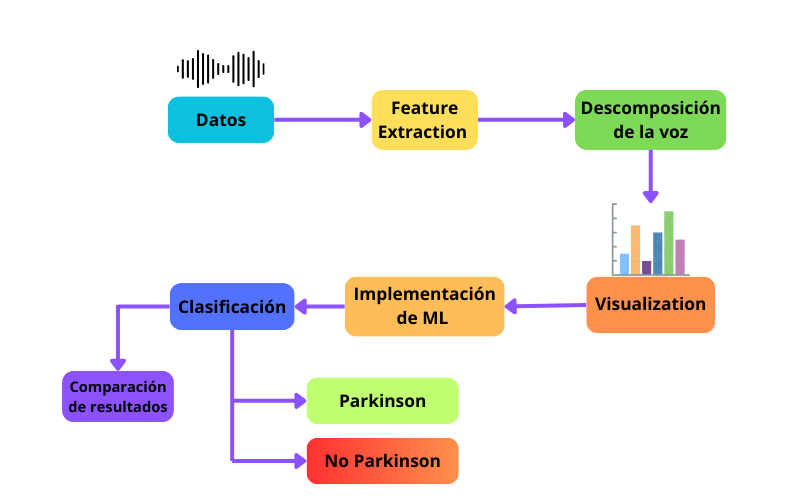
\includegraphics[width=\textwidth]{Datos.png}
    \caption{Diagrama metodológico para la detección de Parkinson utilizando grabaciones de voz.}
    \label{fig:diagrama_metodologico}
\end{figure}


La detección de Parkinson a partir de grabaciones de voz es un desafío que combina distintas disciplinas, desde el análisis de señales hasta el aprendizaje automático. Este proceso metodológico busca garantizar la precisión, robustez y eficiencia en la identificación de patrones asociados con la enfermedad. A continuación, se detalla cada etapa del flujo de trabajo empleado, incluyendo la adquisición de datos, su transformación, análisis y clasificación.

\subsection{Adquisición y Preprocesamiento de Datos}
La calidad de los datos es fundamental para el éxito del análisis. Por ello, se sigue un riguroso protocolo para garantizar que las grabaciones obtenidas sean representativas y estén libres de artefactos no deseados.



\subsubsection{Preprocesamiento de las Señales de Voz}
Antes del análisis, las grabaciones deben ser transformadas para eliminar ruido y resaltar características relevantes:
\begin{itemize}
    \item \textbf{Filtrado de ruido:} Se aplica un filtro pasa-bajas para reducir el ruido de fondo y otras frecuencias no relevantes.
    \item \textbf{Segmentación de la señal:} Se divide cada grabación en fragmentos de longitud fija para facilitar el procesamiento posterior.
    \item \textbf{Normalización:} Se ajustan los niveles de amplitud de las señales para garantizar que todas las grabaciones tengan el mismo rango dinámico.
\end{itemize}

\subsection{Extracción de Características}
La extracción de características consiste en transformar las señales de voz en representaciones numéricas que puedan ser analizadas por algoritmos de aprendizaje automático. Este paso es esencial para capturar patrones relevantes en las grabaciones.

\subsubsection{Decomposición de la Voz}
La descomposición de la voz se realiza mediante técnicas avanzadas que permiten analizar su estructura interna:


\subsubsection{Generación del Vector de Características}
Una vez extraídas, las características se organizan en vectores para su análisis:


\subsection{Visualización de Datos}
Antes de proceder con el aprendizaje automático, se realiza una visualización detallada de los datos para comprender su estructura y distribución:
\begin{itemize}
    \item \textbf{Gráficos de barras:} Utilizados para analizar la frecuencia de las características extraídas.
    \item \textbf{Mapas de calor:} Visualización de correlaciones entre diferentes características.
    \item \textbf{Proyecciones 2D/3D:} Representación visual de las relaciones entre datos mediante reducción de dimensionalidad.
\end{itemize}

\subsection{Implementación de Algoritmos de Aprendizaje Automático}
La etapa más crítica del análisis es la implementación de algoritmos de machine learning que clasifiquen las grabaciones de voz. Se emplean diversos enfoques para maximizar la precisión del modelo.

\subsubsection{Modelos Utilizados}
Los algoritmos seleccionados para este trabajo incluyen:
\begin{itemize}
    \item \textbf{Máquinas de Vectores de Soporte (SVM):} Modelo robusto para la clasificación binaria.
    \item \textbf{K-Nearest Neighbors (KNN):} Método basado en la proximidad de los datos en el espacio vectorial.
    \item \textbf{Random Forest:} Modelo de ensamble que combina múltiples árboles de decisión para mejorar la precisión.
    \item \textbf{AdaBoost:} Algoritmo de boosting que optimiza la clasificación combinando clasificadores débiles.
\end{itemize}

\subsubsection{Entrenamiento y Validación}
El entrenamiento y la evaluación de los modelos se llevan a cabo mediante:
\begin{itemize}
    \item \textbf{División del dataset:} Separación en conjuntos de entrenamiento (80\%) y prueba (20\%).
    \item \textbf{Validación cruzada:} Técnica para evaluar el rendimiento del modelo en diferentes subconjuntos del dataset.
    \item \textbf{Optimización de hiperparámetros:} Ajuste de parámetros clave como el kernel en SVM o la profundidad de los árboles en Random Forest.
\end{itemize}

\subsection{Clasificación y Comparación de Resultados}
El resultado del análisis permite clasificar las grabaciones en dos categorías: "Parkinson" y "No Parkinson". Para evaluar el desempeño, se utilizan métricas como:
\begin{itemize}
    \item \textbf{Precisión:} Porcentaje de clasificaciones correctas.
    \item \textbf{Sensibilidad:} Capacidad del modelo para identificar correctamente los casos positivos.
    \item \textbf{Especificidad:} Habilidad para detectar correctamente los casos negativos.
    \item \textbf{AUC-ROC:} Área bajo la curva que resume el rendimiento general del modelo.
\end{itemize}

\subsection{Interpretación y Resultados Finales}
Los resultados obtenidos son analizados y comparados para extraer conclusiones relevantes:
\begin{itemize}
    \item \textbf{Identificación de patrones:} Relación entre características de voz y la enfermedad de Parkinson.
    \item \textbf{Propuestas de mejora:} Posibles ajustes en la metodología para incrementar la precisión en futuros estudios.
    \item \textbf{Impacto clínico:} Implicaciones de los resultados en el diagnóstico temprano de Parkinson.
\end{itemize}






\begin{thebibliography}{99}

\bibitem{marras2020}
Marras, C., et al. (2020). The natural history of Parkinson's disease: From preclinical stage to motor complications. \textit{Movement Disorders}, 35(5), 821--823. \url{https://doi.org/10.1002/mds.27932}

\bibitem{klein2006}
Klein, C., \& Schlossmacher, M. G. (2006). The genetics of Parkinson disease: Implications for neurological care. \textit{Nature Clinical Practice Neurology}, 2(3), 136--146. \url{https://doi.org/10.1038/ncpneuro0125}

\bibitem{lang1998}
Lang, A. E., \& Lozano, A. M. (1998). Parkinson’s disease: First of two parts. \textit{New England Journal of Medicine}, 339(15), 1044--1053. \url{https://doi.org/10.1056/NEJM199810083391506}

\bibitem{delong1990}
DeLong, M. R. (1990). Primate models of movement disorders of basal ganglia origin. \textit{Trends in Neurosciences}, 13(7), 281--285. \url{https://doi.org/10.1016/0166-2236(90)90110-V}

\bibitem{oms2021}
Organización Mundial de la Salud. (2021). Global Status Report on Parkinson’s Disease. \url{https://www.who.int/publications}

\bibitem{li2021}
Li, J., et al. (2021). Voice-based detection of Parkinson's disease through machine learning. \textit{Biomedical Signal Processing and Control}, 66, 102404. \url{https://doi.org/10.1016/j.bspc.2020.102404}

\bibitem{parkinson1817}
Parkinson, J. (1817). \textit{An Essay on the Shaking Palsy}. Sherwood, Neely, and Jones.

\bibitem{charcot1861}
Charcot, J.-M., \& Vulpain, A. (1861). Sur la paralysie agitante. \textit{Archives de Physiologie Normale et Pathologique}, 4, 149--175.

\bibitem{incn2022}
Instituto Nacional de Ciencias Neurológicas. (2022). Estadísticas sobre el Parkinson en el Perú. \url{https://www.incn.gob.pe}

\bibitem{ali2023}
Ali, A. M., Salim, F., \& Saeed, F. (2023). Parkinson's Disease Detection Using Filter Feature Selection and a Genetic Algorithm with Ensemble Learning. \textit{Diagnostics (Basel, Switzerland)}, 13(17), 2816. \url{https://doi.org/10.3390/diagnostics13172816}

\bibitem{chintalapudi2023}
Chintalapudi, N., Dhulipalla, V. R., Battineni, G., Rucco, C., \& Amenta, F. (2023). Voice Biomarkers for Parkinson’s Disease Prediction Using Machine Learning Models with Improved Feature Reduction Techniques. \textit{Journal of Data Science and Intelligent Systems}. \url{https://doi.org/10.47852/bonviewJDSIS3202831}

\bibitem{islam2024}
Islam, Md S., Adnan, T., Freyberg, J., Lee, S., Abdelkader, A., Pawlik, M., Schwartz, C., Jaffe, K., Schneider, R., Dorsey, E., \& Hoque, E. (2024). Accessible, At-Home Detection of Parkinson's Disease via Multi-task Video Analysis. \textit{arXiv preprint}. \url{https://doi.org/10.48550/arXiv.2406.14856}



\bibitem{terriza2022}
Terriza, M., Navarro, J., Retuerta, I., Alfageme, N., San-Segundo, R., Kontaxakis, G., Garcia-Martin, E., Marijuan, P. C., \& Panetsos, F. (2022). Use of Laughter for the Detection of Parkinson's Disease: Feasibility Study for Clinical Decision Support Systems, Based on Speech Recognition and Automatic Classification Techniques. \textit{International Journal of Environmental Research and Public Health}, 19(17), 10884. \url{https://doi.org/10.3390/ijerph191710884}

\bibitem{alnefaie2024}
Al-Nefaie, A. H., Aldhyani, T. H. H., \& Koundal, D. (2024). Developing System-based Voice Features for Detecting Parkinson’s Disease Using Machine Learning Algorithms. \textit{JDR}, 3(1). \doi{10.57197/JDR-2024-0001}.

\bibitem{srinivasan2024}
Srinivasan, S., Ramadass, P., Mathivanan, S., et al. (2024). Detection of Parkinson disease using multiclass machine learning approach. \textit{Scientific Reports}, 14, 13813. \url{https://doi.org/10.1038/s41598-024-64004-9}

\end{thebibliography}




\end{document}
